\chapter{网络与信息流程分析}
\label{chap:1}

本章針對在深圳研究院的 WLAN 中,从请求接入开始,分别 HTTP 应用以及一种 HTTPS ,並使用 Wireshark 网络抓包工具,进行抓包,并对抓取的信息流程进行分析,试论 Wi-Fi 探针的原理与应用。而本作業在過程中所面對的的問題如下五個章節分別進行說明,首先講述在 Windows 平台上進行 Wireshark 工具安装,其二使用 XAMPP 框架使用 PHP 跟 APACHE 進行測試,其三是在 Mac 平台上使用 Wireshark 工具分析 HTTP 与 HTTPS 的網頁應用,最後在說明 WiFi 探针。


\section{Wireshark 工具安装与说明}

本作业此节说明 Wireshark 工具安装与使用,该节使用的平台为 Windows ,在官网下载安装指定的 Windows 方案,其版本是 Wireshark 3.6.3 64 位元,此外在安装的程序中额外选择了 Npcap 1.55 和 USBPcap 1.5.4.0。安装成后可看到有波动的网路流量,则是可以分析的目标。进入后则是可以看到整体个流量的状况,同时使用 Windows 平台下的命令提示字元去 Ping GitHub Page,来查看封包状况。

\begin{figure}[htb]
\centering 
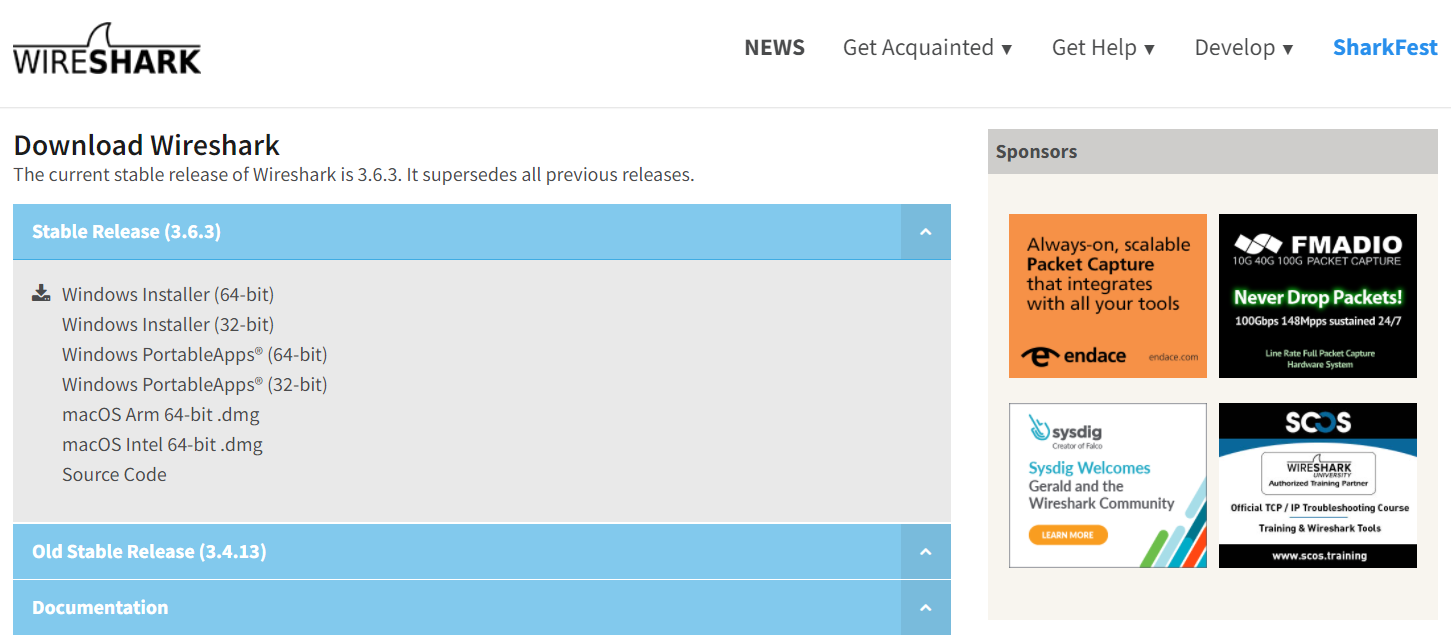
\includegraphics[width=0.90\textwidth]{img/ch1s1m1.png} 
\caption{Wireshark 官方网站}
\label{Test}
\end{figure}

Wireshark 最早名为 Ethereal,其溯源于 1997 年底的一位密苏里大学堪萨斯分校毕业生杰拉德·康姆斯 (Gerald Combs) 在一家小型的网际网路服务供应商上班,他因工作需求,迫切需要一个能够追踪网路流量的工具软体辅助其工作故而开始撰写。在经过几次中断开发的事件过后,于在 1998 年 7 月释出其第一个版本。此后康姆斯收到了来自全世界的修补程式、错误回报与鼓励信件。而 Ethereal 的发展就此而始。不久之后,Gilbert Ramirez 看到了这套软体的开发潜力并开始参予低阶程式的开发。 1998年10月,来自 Network Appliance 公司的 Guy Harris 在寻找一套也是网路封包撷取 tcpview 更好的工具,于是他也开始参与 Ethereal 的开发工作。 1998 年底,一位在教授 TCP/IP 课程的讲师 Richard Sharpe,看到了这套软体的发展潜力,而后开始参与开发与加入新协定的功能。在当时,新的通讯协定的制定并不复杂,因此他开始在Ethereal上新增的封包撷取功能,几乎包含了当时所有通讯协定。自此之后,数以千计的人开始参与 Ethereal的开发,多半是因为希望能让 Ethereal 撷取特定的、尚未包含在 Ethereal 预设的网路协定的封包而参予新的开发,最后 2006 年因商标的问题,Ethereal更名为 Wireshark。

\begin{figure}[htb]
\centering 
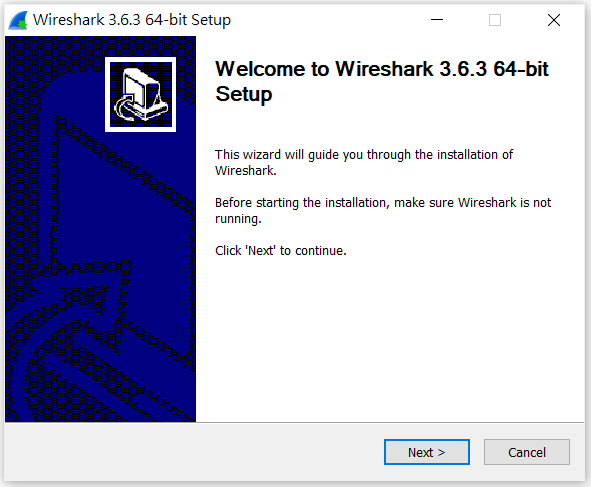
\includegraphics[width=0.60\textwidth]{img/ch1s1m2.png} 
\caption{Wireshark Windows 应用程式安装流程}
\label{Test}
\end{figure}

Npcap 是 Nmap 项目的用于 Microsoft Windows 的数据包捕获和发送库,其本身使用定制的 Windows 内核驱动程序以及 Windows 构建的优秀 libpcap 库来实现开放的 Pcap API。这允许 Windows 软件使用简单、可移植的 API 捕获包括无线网络、有线以太网、本地主机流量和许多 VPN 等原始网络流量。 Npcap 也允许发送原始数据包,因为 Mac 和 Linux 系统已经包含 Pcap API,因此 Npcap 允许流行的软件,例如 Nmap 和 Wireshark 使用单个代码库在所有这些平台上运行。其 Npcap 最早始于 2013 年,作为对现已停止的 WinPcap 库的一些改进,但与之差别的是从那时起,前者已在很大程度上被重写,经过数百个版本提高了 Npcap 的速度、可移植性、安全性和效率。

\begin{figure}[htb]
\centering 
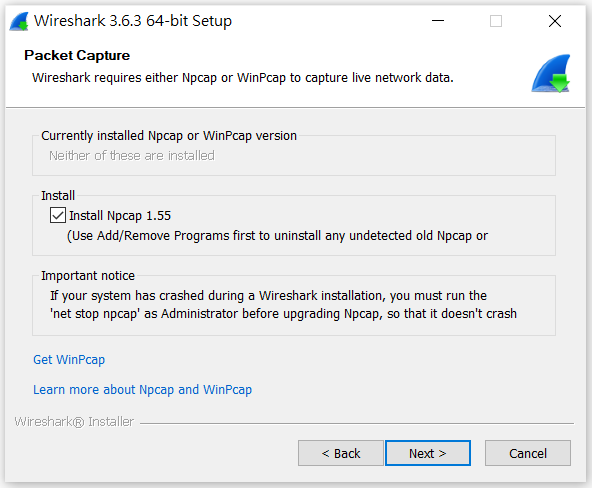
\includegraphics[width=0.60\textwidth]{img/ch1s1m3.png} 
\caption{Install Npcap 1.55}
\label{Test}
\end{figure}

\begin{figure}[htb]
\centering 
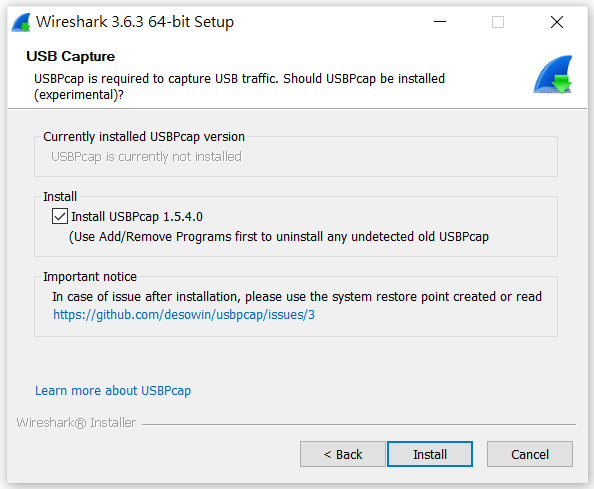
\includegraphics[width=0.60\textwidth]{img/ch1s1m4.png} 
\caption{Install USBPcap 1.5.4.0}
\label{Test}
\end{figure}

\begin{figure}[htb]
\centering 
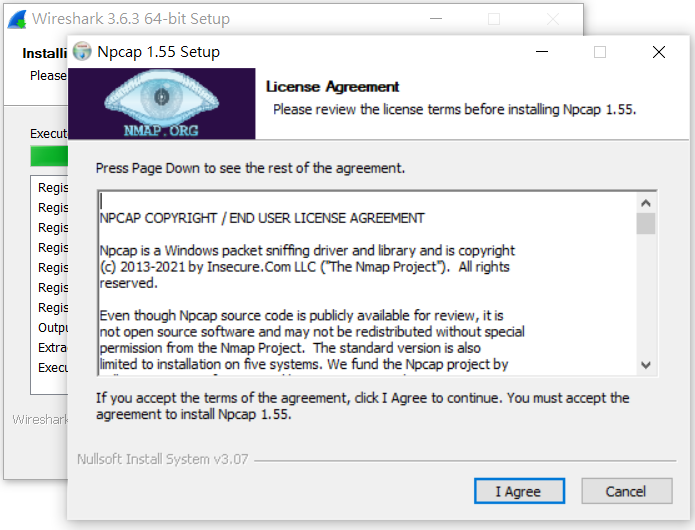
\includegraphics[width=0.60\textwidth]{img/ch1s1m5.png} 
\caption{Npcap 1.55 流程}
\label{Test}
\end{figure}

\begin{figure}[htb]
\centering 
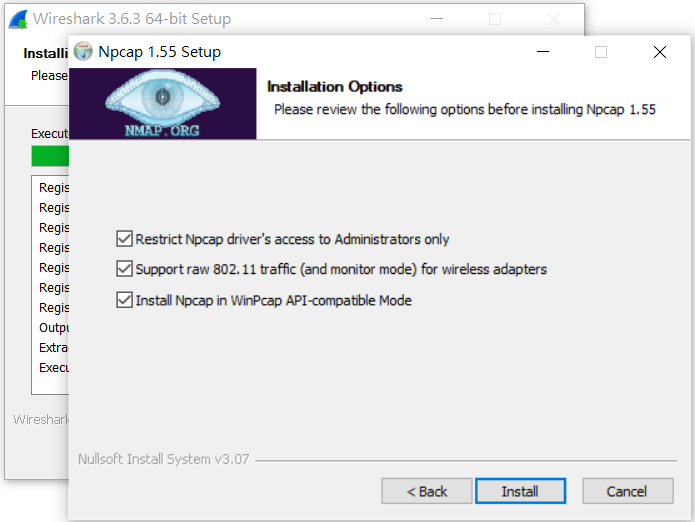
\includegraphics[width=0.60\textwidth]{img/ch1s1m6.png} 
\caption{Npcap 1.55 设定}
\label{Test}
\end{figure}

USBPcap 是可以让 Wireshark 来获得 Windows 的 USB 数据包,前者可以让后者能够对来自 USB 的封包进行分析,同样地该工具也是开源许可。

\begin{figure}[htb]
\centering 
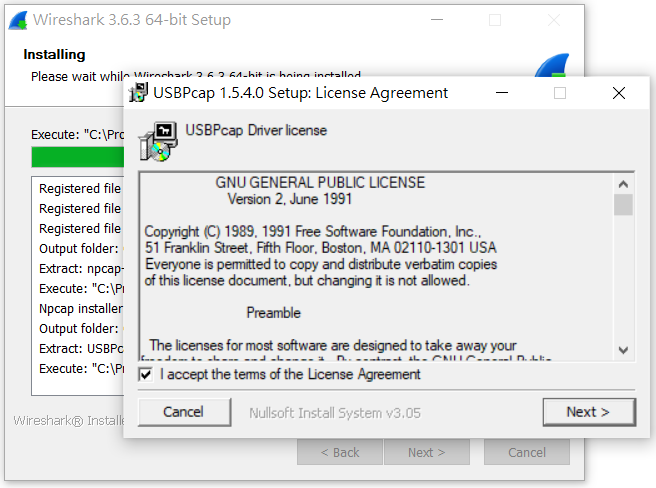
\includegraphics[width=0.60\textwidth]{img/ch1s1m7.png} 
\caption{USBPcap 1.5.4.0 流程}
\label{Test}
\end{figure}

\begin{figure}[htb]
\centering 
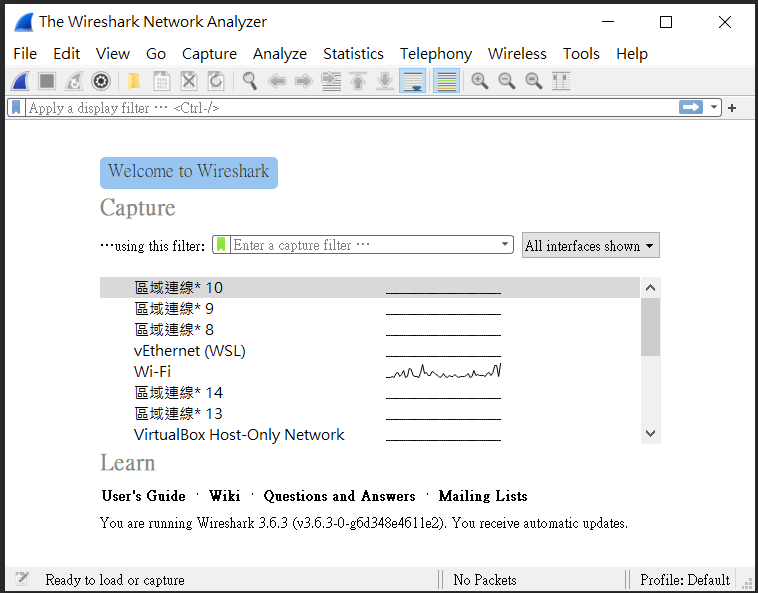
\includegraphics[width=0.70\textwidth]{img/ch1s1m8.png} 
\caption{Wireshark 应用程式画面}
\label{Test}
\end{figure}

\begin{figure}[htb]
\centering 
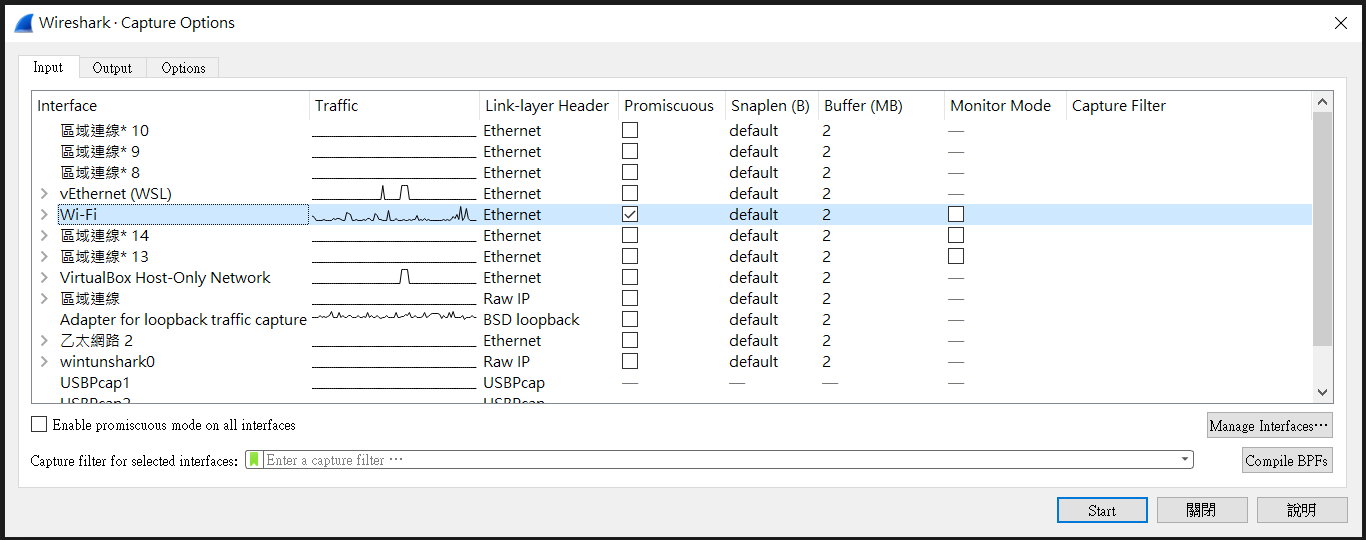
\includegraphics[width=0.90\textwidth]{img/ch1s1m9.png} 
\caption{Wireshark 封包选项}
\label{Test}
\end{figure}

\begin{figure}[htb]
\centering 
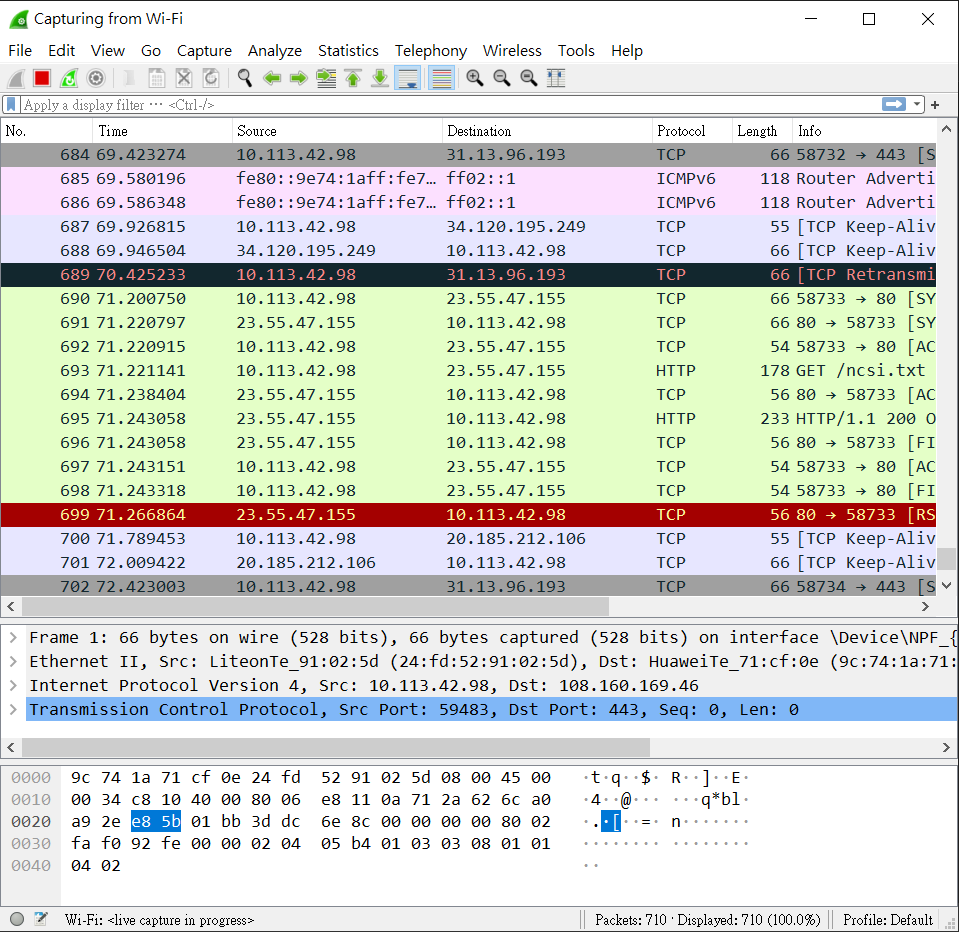
\includegraphics[width=0.90\textwidth]{img/ch1s1m10.png} 
\caption{WiFi 追踪}
\label{Test}
\end{figure}

在本节可以看到 Windows 平台的 Wireshark 顺利的进行安装,同时对 GitHub Page 进行分析,所谓的 GitHub Page 是开放原始码的版本控制平台 GitHub ,其所提供的静态页面服务,多用于该开源项目或者使用者进行项目的展示与说明之用。从分析过程中可以看到 Wireshark 顺利的侦测到 GitHub Page 的状态,后面本作业会尝试说明 OpenSSL 与 CA 的设定。

\begin{Verbatim}
> ping kancheng.github.io
\end{Verbatim}

\begin{figure}[htb]
\centering 
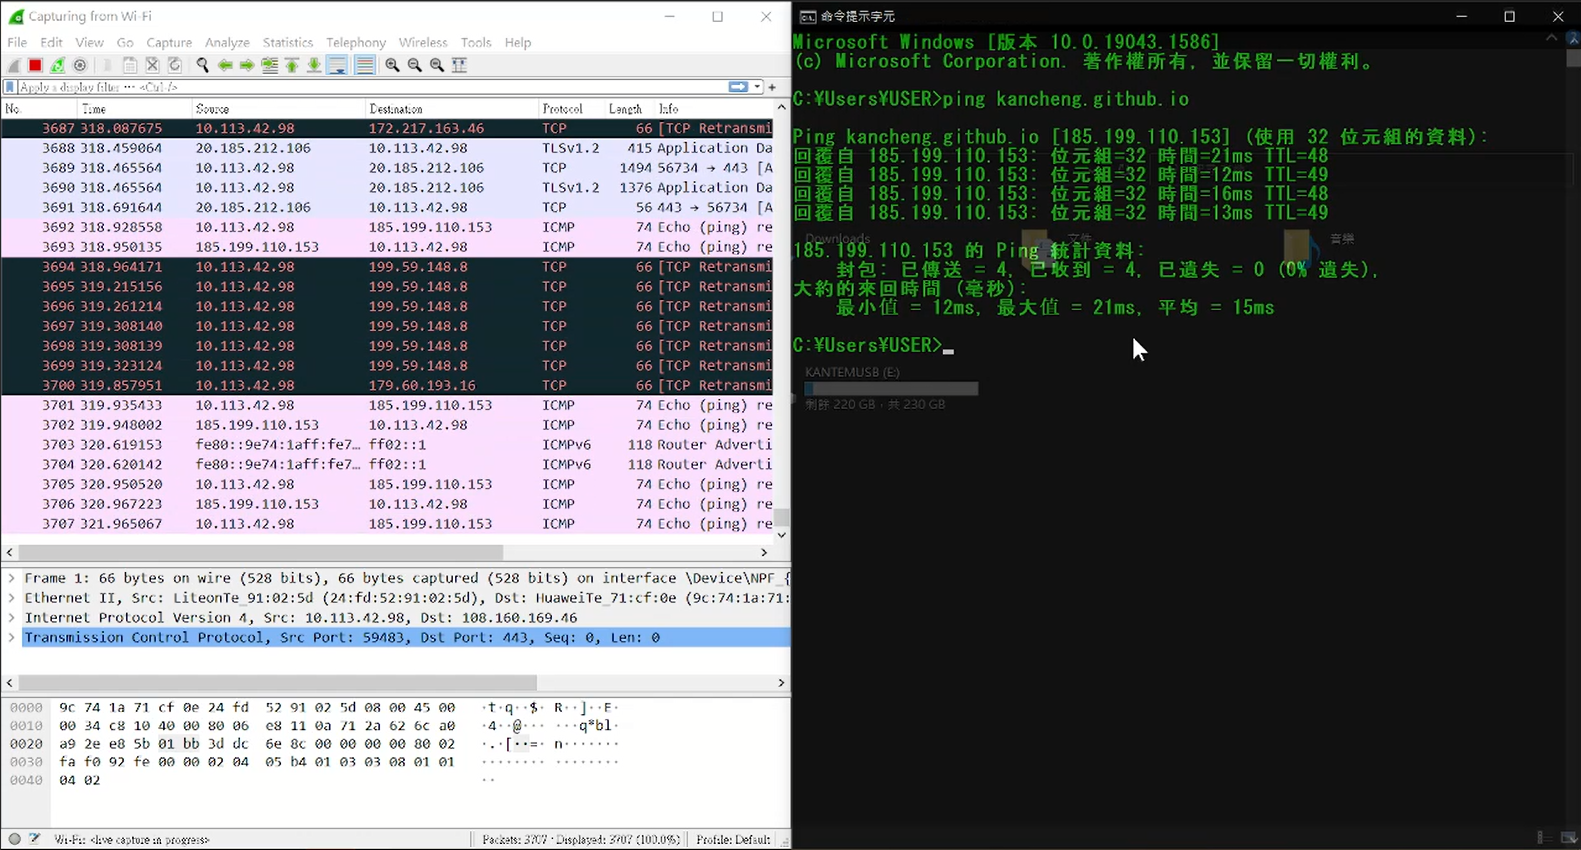
\includegraphics[width=0.90\textwidth]{img/ch1s1m11.png} 
\caption{使用 GitHub Page 测试}
\label{Test}
\end{figure}

\section{Linux tcpdump 封包分析}

在网络问题的调试中,tcpdump 应该说是一个必不可少的工具和大部分 Linux 下的优秀工具一样,它的特点就是简单而强大。它是基于 Unix 系统的命令行式的数据包嗅探工具,可以抓取流动在网卡上的数据包。默认情况下,tcpdump不会抓取本机内部通讯的报文。根据网络协议栈的规定,对于报文,即使是目的地是本机,也需要经过本机的网络协议层,所以本机通讯肯定是通过API进入了内核,并且完成了路由选择,比如本机的 TCP 通信,也必须要有 Socket 通信的基本要素。如果要使用 tcpdump 抓取其他主机 MAC 地址的数据包,必须开启网卡混杂模式,所谓混杂模式,用最简单的语言就是让网卡抓取任何经过它的数据包,不管这个数据包是不是发给它或者是它发出的。一般而言,Unix 不会让普通用户设置混杂模式,因为这样可以看到别人的信息,比如 telnet 的用户名和密码,这样会引起一些安全上的问题,所以只有 root 用户可以开启混杂模式,开启混杂模式的命令是:ifconfig en0 promisc, 而 en0 则是假设所要打开混杂模式的网卡。


\subsection{Linux 抓包原理}

Linux 抓包是通过注册一种虚拟的底层网络协议来完成对网络报文,准确来说是网络设备的消息处理权。当网卡接收到一个网络报文之后,它会遍历系统中所有已经注册的网络协议,例如以太网协议、 x25 协议处理模块来尝试进行报文的解析处理,这一点和一些文件系统的挂载相似,就是让系统中所有的已经注册的文件系统来进行尝试挂载,如果哪一个认为自己可以处理,那么就完成挂载。当抓包模块把自己伪装成一个网络协议的时候,系统在收到报文的时候就会给这个伪协议一次机会,让它来对网卡收到的报文进行一次处理,此时该模块就会趁机对报文进行窥探,也就是把这个报文完完整整的复制一份,假装是自己接收到的报文,汇报给抓包模块。当然 Wireshark 是一个网络协议检测工具,支持 Windows 平台、 Unix 平台、 Mac 平台,一般只在图形界面平台下使用 Wireshark,如果是 Linux 的话,则可直接使用 tcpdump,因为一般而言 Linux 都自带的 tcpdump ,或者用 tcpdump 抓包以后用 Wireshark 打开分析。而在 Mac 平台下, Wireshark 通过 WinPcap 进行抓包,且封装跟使用方便,可很容易的制定抓包过滤器或者显示过滤器。两者相比,tcpdump 是用来抓取数据非常方便,Wireshark 则是用于分析抓取到的数据比较方便。

%\begin{Verbatim}

%\end{Verbatim}

\begin{Verbatim}
tcpdump [-adeflnNOpqStvx][-c<数据包数目>]
[-dd][-ddd][-F<表达文件>][-i<网络界面>]
[-r<数据包文件>][-s<数据包大小>][-tt]
[-T<数据包类型>][-vv][-w<数据包文件>][输出数据栏位]
\end{Verbatim}

\begin{itemize}
\item [-] -a 尝试将网络和广播地址转换成名称。
\item [-] -c <数据包数目> 收到指定的数据包数目后,就停止进行倾倒操作。
\item [-] -d 把编译过的数据包编码转换成可阅读的格式,并倾倒到标准输出。
\item [-] -dd 把编译过的数据包编码转换成C语言的格式,并倾倒到标准输出。
\item [-] -ddd 把编译过的数据包编码转换成十进制数字的格式,并倾倒到标准输出。
\item [-] -e 在每列倾倒资料上显示连接层级的文件头。
\item [-] -f 用数字显示网际网络地址。
\item [-] -F <表达文件> 指定内含表达方式的文件。
\item [-] -i <网络界面> 使用指定的网络截面送出数据包。
\item [-] -l 使用标准输出列的缓冲区。
\item [-] -n 不把主机的网络地址转换成名字。
\item [-] -N 不列出域名。
\item [-] -O 不将数据包编码最佳化。
\item [-] -p 不让网络界面进入混杂模式。
\item [-] -q 快速输出,仅列出少数的传输协议信息。
\item [-] -r <数据包文件> 从指定的文件读取数据包数据。
\item [-] -s <数据包大小> 设置每个数据包的大小。
\item [-] -S 用绝对而非相对数值列出TCP关联数。
\item [-] -t 在每列倾倒资料上不显示时间戳记。
\item [-] -tt 在每列倾倒资料上显示未经格式化的时间戳记。
\item [-] -T <数据包类型> 强制将表达方式所指定的数据包转译成设置的数据包类型。
\item [-] -v 详细显示指令执行过程。
\item [-] -vv 更详细显示指令执行过程。
\item [-] -x 用十六进制字码列出数据包资料。
\item [-] -w <数据包文件> 把数据包数据写入指定的文件。
\end{itemize}

\begin{figure}[htb]
\centering 
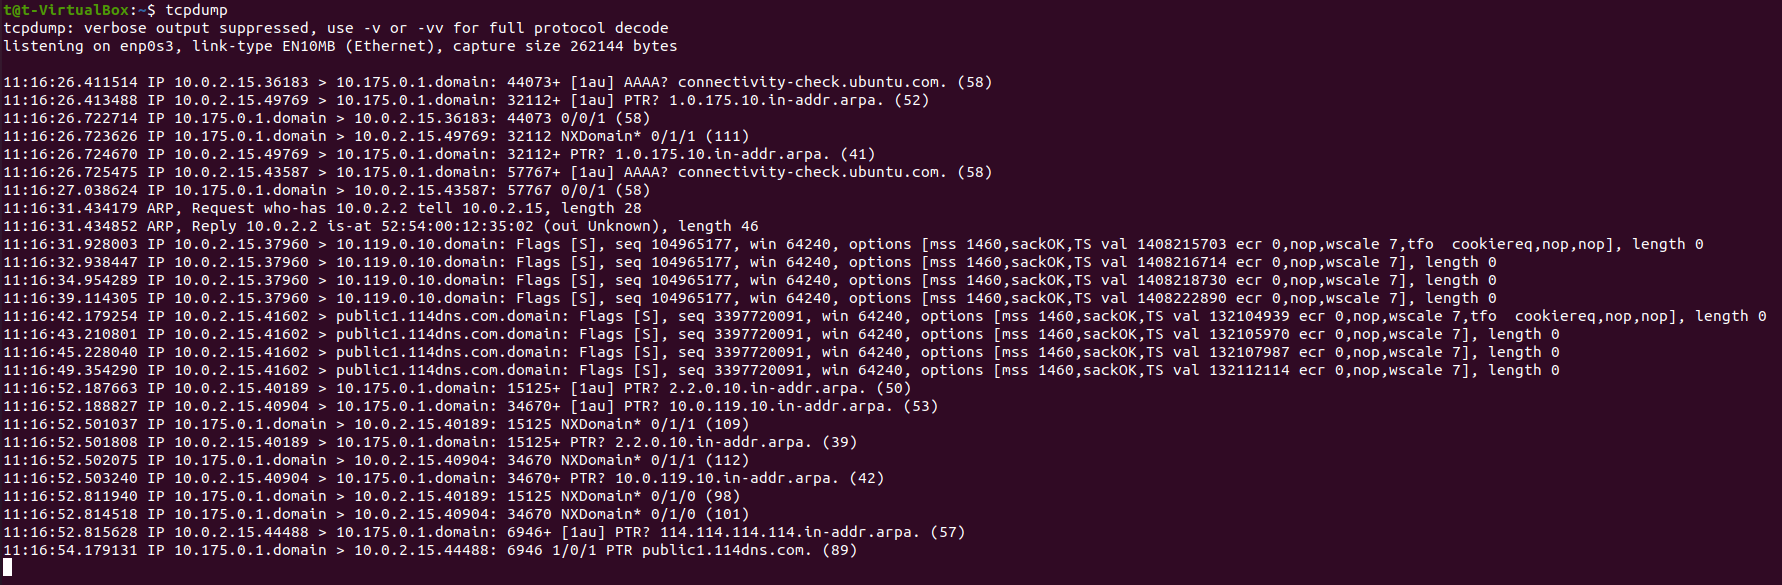
\includegraphics[width=0.80\textwidth]{img/newch1m1.png} 
\caption{tcpdump}
\label{Test}
\end{figure}

\begin{Verbatim}
$ # 1. 显示 TCP 包信息
$ tcpdump
$ # 2. 显示指定数量包
$ tcpdump -c 20
$ # 3. 精简显示
$ tcpdump -c 10 -q //精简模式显示 10个包
$ # 4. 转换克阅读格式
$ tcpdump -d
$ # 5. 转换成十进制格式
$ tcpdump -ddd
$ # 6. 通过 tcpdump 截获主机 www.baidu.com 发送与接收所有的数据包
$ tcpdump -i en0 host www.baidu.com
$ sudo tcpdump -i en0 host www.baidu.com
\end{Verbatim}

\subsection{tcpdump 抓取 TCP 包分析}

TCP 传输控制协议是面向连接的可靠的传输层协议,在进行数据传输之前,需要在传输数据的两端,也就是客户端和服务器端中创建一个连接,这个连接由一对插口地址唯一标识,即是在IP报文首部的源IP地址、目的 IP 地址,以及TCP数据报首部的源端口地址和目的端口地址。其 TCP 首部结构如下。

\begin{figure}[htb]
\centering 
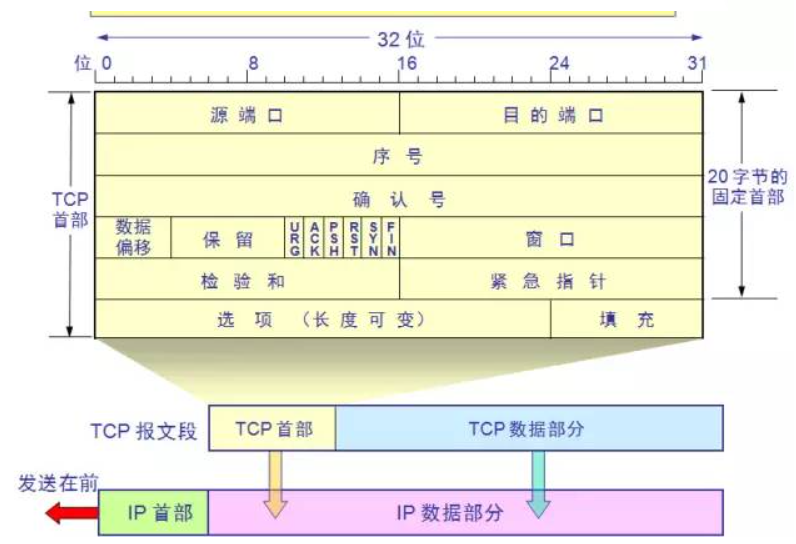
\includegraphics[width=0.80\textwidth]{img/newch1m2.png} 
\caption{tcpdump}
\label{Test}
\end{figure}

同時要注意在通常情况下,一个正常的 TCP 连接,都会有三个阶段,也就是 1、TCP三次握手; 2、数据传送; 3、TCP四次挥手,其中在 TCP 连接和断开连接过程中的关键部分如下:

\begin{itemize}
\item [-] 源端口号:即发送方的端口号,在TCP连接过程中,对于客户端,端口号往往由内核分配,无需进程指定;
\item [-] 目的端口号:即发送目的的端口号;
\item [-] 序号:即为发送的数据段首个字节的序号;
\item [-] 确认序号:在收到对方发来的数据报,发送确认时期待对方下一次发送的数据序号;
\item [-] SYN:同步序列编号,Synchronize Sequence Numbers;
\item [-] ACK:确认编号,Acknowledgement Number;
\item [-] FIN:结束标志,FINish;
\end{itemize}

\subsection{TCP 三次握手}

\begin{figure}[htb]
\centering 
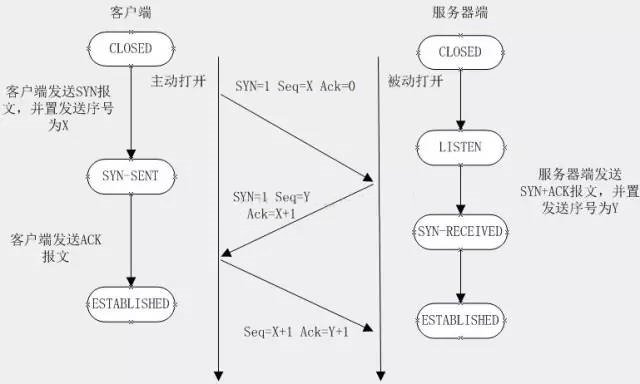
\includegraphics[width=0.80\textwidth]{img/newch1m3.png} 
\caption{TCP 三次握手}
\label{Test}
\end{figure}

三次握手的过程如下:

\begin{itemize}
\item [-] Step1. 由客户端向服务器端发起 TCP 连接请求。 Client 发送:同步序列编号SYN置为1,发送序号 Seq 为一个随机数,这里假设为 X,确认序号 ACK 置为 0;
\item [-] Step2. 服务器端接收到连接请求。 Server 响应,其同步序列编号SYN置为1,并将确认序号 ACK 置为 X+1,然后生成一个随机数Y作为发送序号 Seq (因为所确认的数据报的确认序号未初始化);
\item [-] Step3. 客户端对接收到的确认进行确认。 Client 发送,将确认序号 ACK 置为 Y+1,然后将发送序号 Seq 置为 X+1(即为接收到的数据报的确认序号);
\end{itemize}

至于为什么是三次握手而不是两次对于 Step3 的作用,假设一种情况,客户端A向服务器B发送一个连接请求数据报,然后这个数据报在网络中滞留导致其迟到了,虽然迟到了,但是服务器仍然会接收并发回一个确认数据报。但是A却因为久久收不到 B 的确认而将发送的请求连接置为失效,等到一段时间后,接到B发送过来的确认,A认为自己现在没有发送连接,而B却一直以为连接成功了,于是一直在等待A的动作,而A将不会有任何的动作了。这会导致服务器资源白白浪费掉了,因此,两次握手是不行的,因此需要再加上一次,对B发过来的确认再进行一次确认,即确认这次连接是有效的,从而建立连接。对于双方,发送序号的初始化为何值有的系统中是显式的初始化序号是0,但是这种已知的初始化值是非常危险的,因为这会使得一些黑客钻漏洞,发送一些数据报来破坏连接。因此,初始化序号因为取随机数会更好一些,并且是越随机越安全。

\subsection{TCP 四次握手}

\begin{figure}[htb]
\centering 
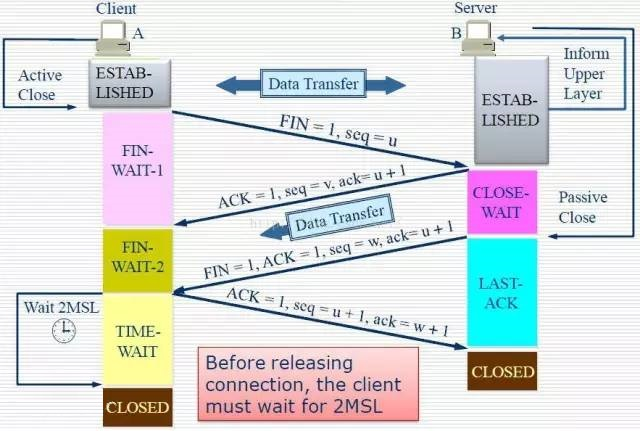
\includegraphics[width=0.80\textwidth]{img/newch1m4.png} 
\caption{TCP 四次握手}
\label{Test}
\end{figure}

连接双方在完成数据传输之后就需要断开连接。由于TCP连接是属于全双工的,即连接双方可以在一条TCP连接上互相传输数据,因此在断开时存在一个半关闭状态,即有有一方失去发送数据的能力,却还能接收数据。因此,断开连接需要分为四次。主要过程如下:

\begin{itemize}
\item [-] Step1. 主机 A 向主机B发起断开连接请求,之后主机 A 进入 FIN-WAIT-1 状态;
\item [-] Step2. 主机 B 收到主机 A 的请求后,向主机 A 发回确认,然后进入 CLOSE-WAIT 状态;
\item [-] Step3. 主机 A 收到 B 的确认之后,进入 FIN-WAIT-2 状态,此时便是半关闭状态,即主机A失去发送能力,但是主机B却还能向A发送数据,并且 A 可以接收数据。此时主机 B 占主导位置了,如果需要继续关闭则需要主机B来操作了;
\item [-] Step4. 主机 B 向 A 发出断开连接请求,然后进入 LAST-ACK 状态;
\item [-] Step5. 主机 A 接收到请求后发送确认,进入 TIME-WAIT 状态,等待 2MSL 之后进入 CLOSED 状态,而主机B则在接受到确认后进入 CLOSED 状态;
\end{itemize}

为何主机 A 在发送了最后的确认后没有进入 CLOSED 状态,反而进入了一个等待 2MSL 的 TIME-WAIT 主要作用有两个:第一,确保主机A最后发送的确认能够到达主机B。如果处于LAST-ACK状态的主机B一直收不到来自主机A的确认,它会重传断开连接请求,然后主机A就可以有足够的时间去再次发送确认。但是这也只能尽最大力量来确保能够正常断开,如果主机A的确认总是在网络中滞留失效,从而超过了2MSL,最后也无法正常断开;第二,如果主机A在发送了确认之后立即进入CLOSED状态。假设之后主机A再次向主机B发送一条连接请求,而这条连接请求比之前的确认报文更早地到达主机B,则会使得主机B以为这条连接请求是在旧的连接中A发出的报文,并不看成是一条新的连接请求了,即使得这个连接请求失效了,增加2MSL的时间可以使得这个失效的连接请求报文作废,这样才不影响下次新的连接请求中出现失效的连接请求。为什么断开连接请求报文只有三个,而不是四个因为在TCP连接过程中,确认的发送有一个延时(即经受延时的确认),一端在发送确认的时候将等待一段时间,如果自己在这段事件内也有数据要发送,就跟确认一起发送,如果没有,则确认单独发送。而我们的抓包实验中,由服务器端先断开连接,之后客户端在确认的延迟时间内,也有请求断开连接需要发送,于是就与上次确认一起发送,因此就只有三个数据报了。

\section{Chrome 封包分析}

所谓的抓包,即抓取本地电脑与远端服务器通信时候所传递的数据包,而 Chrome 开发者工具是一套内置于 Google Chrome 中的 Web 开发和调试工具,可用来对网站进行迭代、调试和分析,
而想要打开 Chrome 开发者工具则是在 Chrome 界面中按下键盘的 F12 键,又或者是在页面元素上右键点击选择后,选取检查。

\begin{figure}[htb]
\centering 
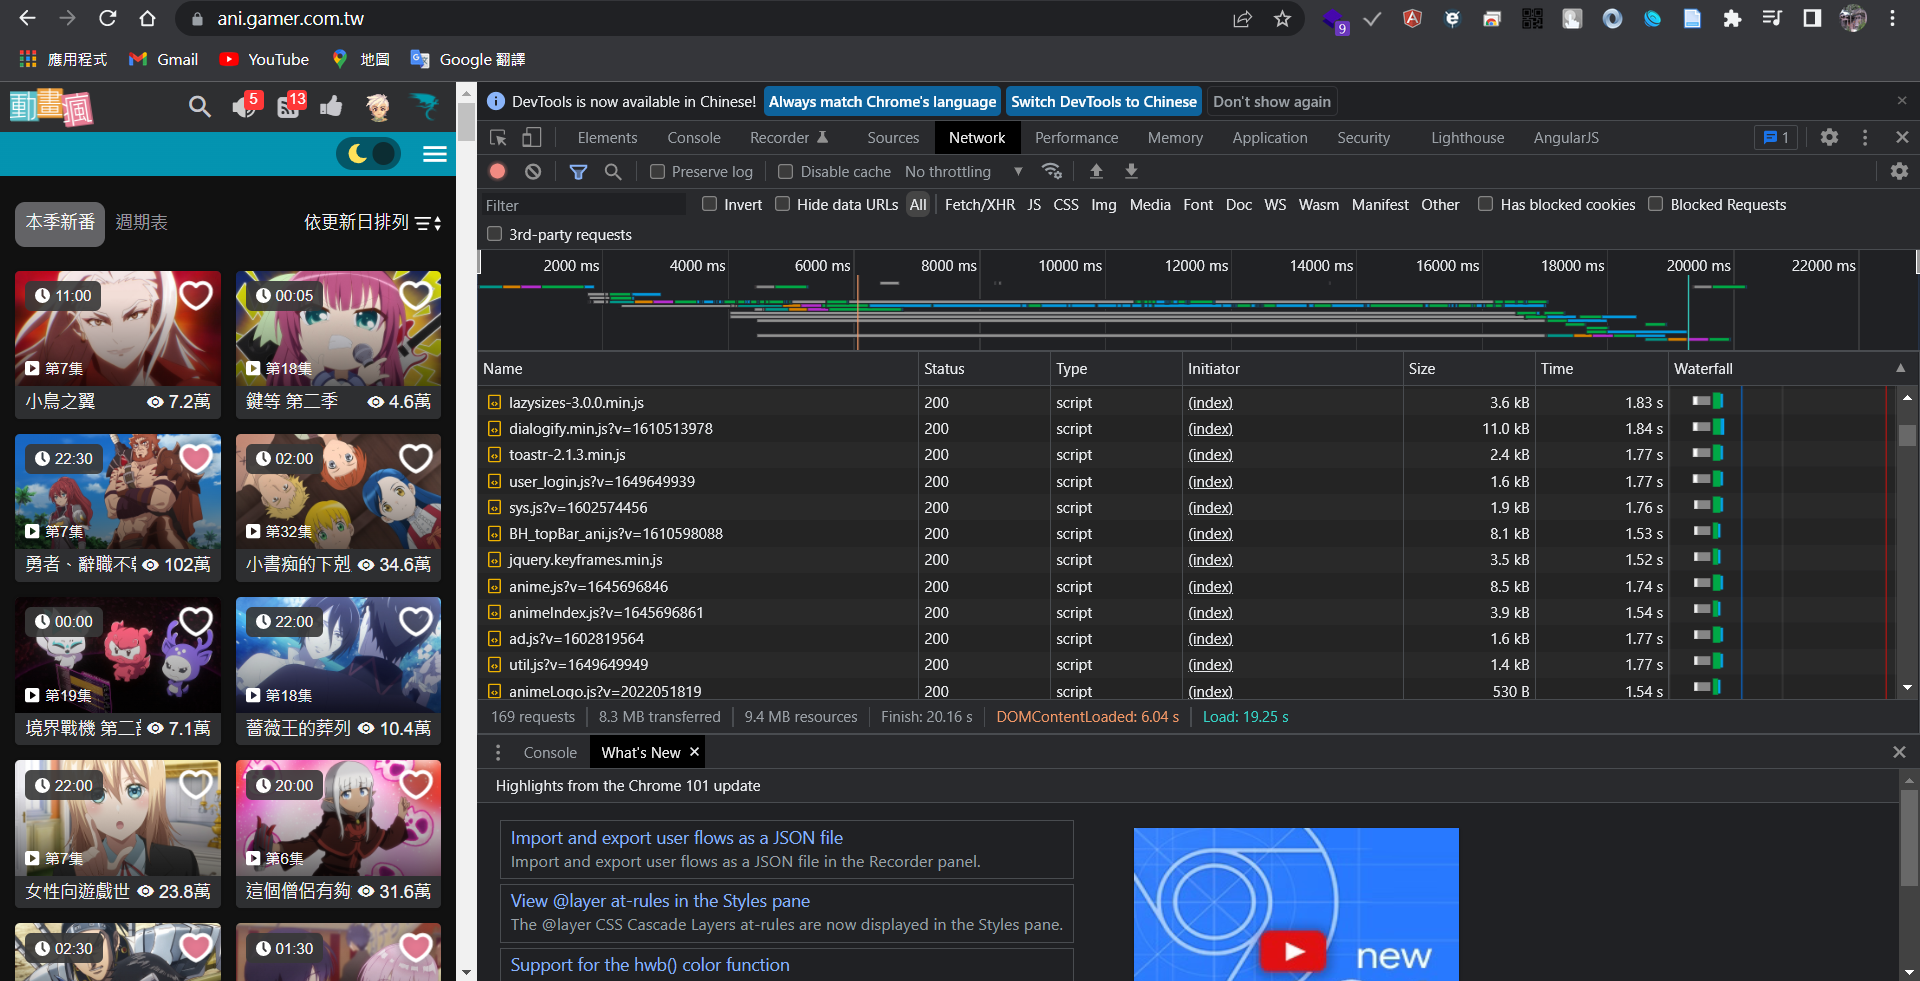
\includegraphics[width=0.80\textwidth]{img/newch1m5.png} 
\caption{Chrome 介面}
\label{Test}
\end{figure}

\subsection{开发者工具的结构}

\begin{figure}[htb]
\centering 
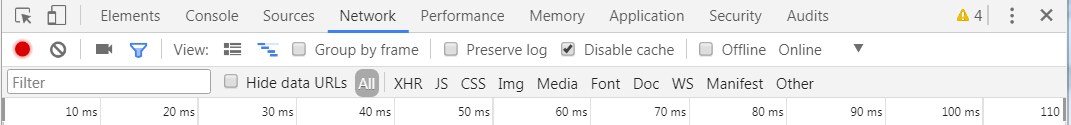
\includegraphics[width=0.80\textwidth]{img/newch1m6.png} 
\caption{Chrome 开发者工具的结构}
\label{Test}
\end{figure}

\begin{itemize}
\item [-] Elements (元素面板):使用“元素”面板可以通过自由操纵 DOM 和 CSS 来重演您网站的布局和设计。
\item [-] Console (控制台面板):在开发期间,可以使用控制台面板记录诊断信息,或者使用它作为 Shell,在页面上与 JavaScript 交互。
\item [-] Sources (源代码面板):在源代码面板中设置断点来调试 JavaScript ,或者通过 Workspaces (工作区) 连接本地文件来使用开发者工具的实时编辑器。
\item [-] Network (网络面板):从发起网页页面请求 Request 后得到的各个请求资源信息,當中包括了状态、资源类型、大小、所用时间等,并可以根据这个进行网络性能优化
\item [-] Performance (性能面板):使用时间轴面板,可以通过记录和查看网站生命周期内发生的各种事件来提高页面运行时的性能
\item [-] Memory (内存面板):分析 Web 应用或者页面的执行时间以及内存使用情况
\item [-] Application (应用面板):记录网站加载的所有资源信息,包括存储数据 (Local Storage、Session Storage、IndexedDB、Web SQL、Cookies)、缓存数据、字体、图片、脚本、样式表等
\item [-] Security (安全面板):使用安全面板调试混合内容问题,证书问题等等
\item [-] Audits (审核面板):对当前网页进行网络利用情况、网页性能方面的诊断,并给出一些优化建议。比如列出所有没有用到的 CSS 文件等
\end{itemize}

\subsection{Network 网络面板}

从开发者工具的结构中可以看到 Network 面板记录页面上每个网络操作的相关信息,包括从发起网页页面请求 Request 后得到的各个请求资源信息,当中包括了状态、资源类型、大小、所用时间等,并可以根据这个进行网络性能优化,看到详细的耗时数据、HTTP 请求与响应标头和 Cookie。该结构由五个窗格组成,包含了控件 (Controls)、过滤器 (Filter)、Overview (概览)、请求列表 (Request Table)、概要 (Summary)。

\begin{figure}[htb]
\centering 
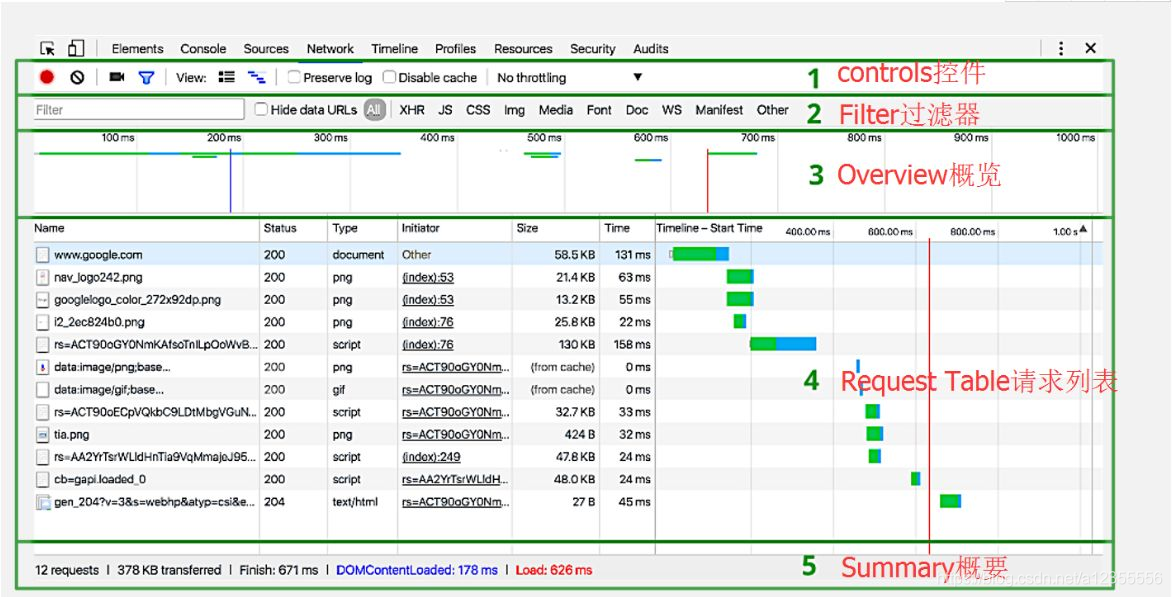
\includegraphics[width=0.80\textwidth]{img/newch1m7.png} 
\caption{Chrome 开发者工具的 Network}
\label{Test}
\end{figure}

\subsection{Controls 控件}

Controls 控件使用记录请求、清除请求、捕获截图、保存日志、禁用缓存等选项,来控制 Network 网络面板的外观和功能。

\begin{figure}[htb]
\centering 
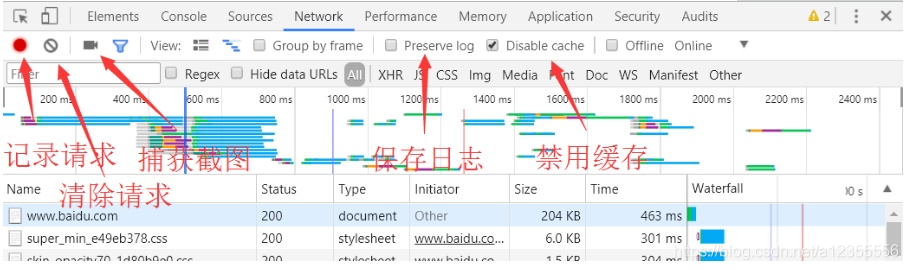
\includegraphics[width=0.80\textwidth]{img/newch1m8.png} 
\caption{Chrome 开发者工具的 Network}
\label{Test}
\end{figure}

\subsection{Filters 过滤器}

Filters 过滤器使用一些选项来控制在请求列表中显示当中的资源,使用上按住键盘的 Ctrl 键(Window / Linux),然后点击过滤器可以同时选择多个过滤器。此外,筛选框可以实现很多定制化的筛选,比如字符串匹配,关键词筛选等,其中关键词筛选主要有如下几种:

\begin{figure}[htb]
\centering 
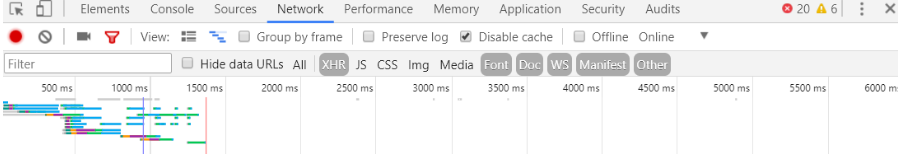
\includegraphics[width=0.80\textwidth]{img/newch1m9.png} 
\caption{Chrome 开发者工具的 Filters}
\label{Test}
\end{figure}

\begin{itemize}
\item [-] domain:仅显示来自指定域的资源。您可以使用通配符()来包括多个域。例如 .com 显示以 .com 结尾的所有域名中的资源。 DevTools 会在自动完成下拉菜单中自动填充它遇到的所有域。
\item [-] has-response-header:显示包含指定 HTTP 响应头信息的资源。 DevTools 会在自动完成下拉菜单中自动填充它遇到的所有响应头。
\item [-] is:通过 is:running 找出 WebSocket 请求。
\item [-] larger-than (大于) :显示大于指定大小的资源(以字节为单位)。设置值 1000 等效于设置值 1k。
\item [-] method (方法):显示通过指定的 HTTP 方法类型检索的资源。DevTools 使用它遇到的所有 HTTP 方法填充下拉列表。
\item [-] mime-type (mime 类型):显示指定 MIME 类型的资源。 DevTools 使用它遇到的所有 MIME 类型填充下拉列表。
\item [-] mixed-content (混合内容):显示所有混合内容资源(mixed-content:all)或仅显示当前显示的内容(mixed-content:displayed)。
\item [-] Scheme(协议):显示通过不受保护的 HTTP(scheme:http)或受保护的 HTTPS(scheme:https)检索的资源。
\item [-] set-cookie-domain(cookie域):显示具有 Set-Cookie 头,并且其 Domain 属性与指定值匹配的资源。DevTools 会在自动完成下拉菜单中自动填充它遇到的所有 Cookie 域。
\item [-] set-cookie-name(cookie名):显示具有 Set-Cookie 头,并且名称与指定值匹配的资源。DevTools 会在自动完成下拉菜单中自动填充它遇到的所有 Cookie 名。
\item [-] set-cookie-value(cookie值):显示具有 Set-Cookie 头,并且值与指定值匹配的资源。DevTools 会在自动完成下拉菜单中自动填充它遇到的所有cookie值。
\item [-] status-code(状态码):仅显示其 HTTP 状态代码与指定代码匹配的资源。DevTools 会在自动完成下拉菜单中自动填充它遇到的所有状态码。
\end{itemize}

\subsection{Overview 概览}

\begin{figure}[htb]
\centering 
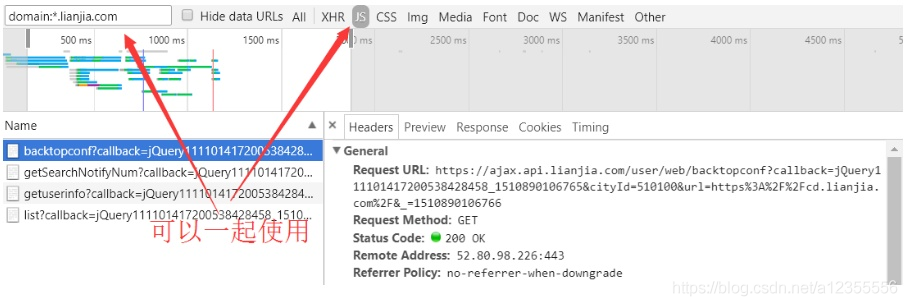
\includegraphics[width=0.80\textwidth]{img/newch1m10.png} 
\caption{Chrome 开发者工具的 Domain 操作}
\label{Test}
\end{figure}

Overview 概览图表显示检索资源的时间轴。如果您看到多个垂直堆叠的栏,这意味着这些资源被同时检索。

\subsection{Requests Table 请求列表}

\begin{figure}[htb]
\centering 
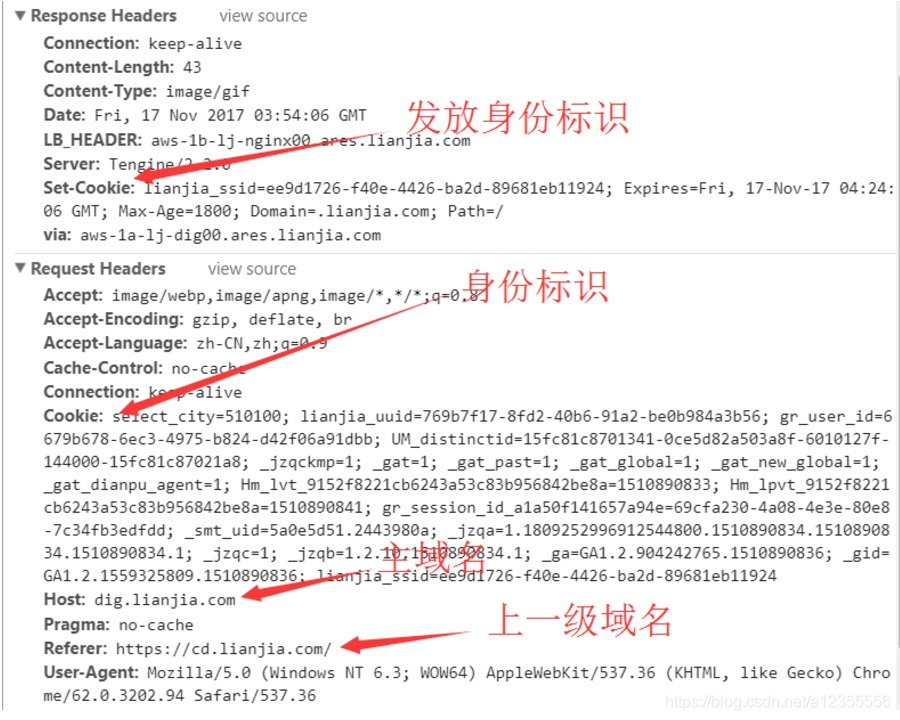
\includegraphics[width=0.80\textwidth]{img/newch1m11.png} 
\caption{Chrome 开发者工具的 Response}
\label{Test}
\end{figure}

Requests Table 的请求列表中列出了检索的每个资源。默认情况下,此表按时间顺序排序,也就是最早的资源在顶部。单击资源名称可以获得更多信息。提示:右键单击列表的任何标题栏可以以添加或删除信息列。

查看单个资源的详细信息,可点击资源名称,其位于 Requests Table 的 Name 列下,可以查看与该资源有关的更多信息。可用标签会因您所选择资源类型的不同而不同,但下面四个标签最常见:

\begin{figure}[htb]
\centering 
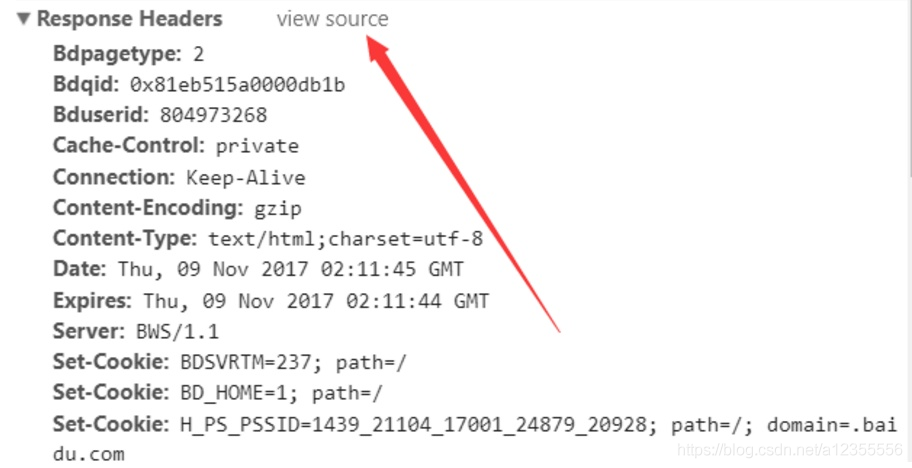
\includegraphics[width=0.80\textwidth]{img/newch1m12.png} 
\caption{Chrome 开发者工具的 Preview}
\label{Test}
\end{figure}

\begin{itemize}
\item [-] Headers:与资源关联的 HTTP 标头。
\item [-] Preview:JSON、图像和文本资源的预览。
\item [-] Response:HTTP 响应数据 (如果存在)。
\item [-] Timing:资源请求生命周期的精细分解。
\item [-] Headers (查看 HTTP 标头) 点击 Headers 可以显示该资源的标头。 Headers 标签可以显示资源的请求网址、HTTP 方法以及响应状态代码。 此外,该标签还会列出 HTTP 响应和请求标头、它们的值以及任何查询字符串参数,点击每一部分旁边的 view source 或 view parsed 链接,您能够以源格式或者解析格式查看响应标头、请求标头或者查询字符串参数。
\item [-] Preview (预览资源) 点击 Preview 标签可以查看该资源的预览。Preview 标签可能显示一些有用的信息,也可能不显示,具体取决于您所选择资源的类型。
\item [-] Response (查看 HTTP 响应内容) 点击 Response 标签可以查看资源未格式化的 HTTP 响应内容。 Preview 标签可能包含一些有用的信息,也可能不包含,具体取决于您所选择资源的类型。
\end{itemize}

\begin{figure}[htb]
\centering 
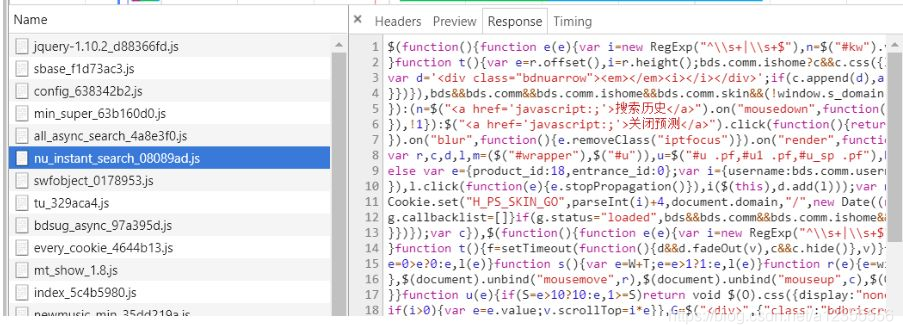
\includegraphics[width=0.80\textwidth]{img/newch1m13.png} 
\caption{Chrome 开发者工具的查看 Response}
\label{Test}
\end{figure}

\subsection{查看 Cookie}

\begin{figure}[htb]
\centering 
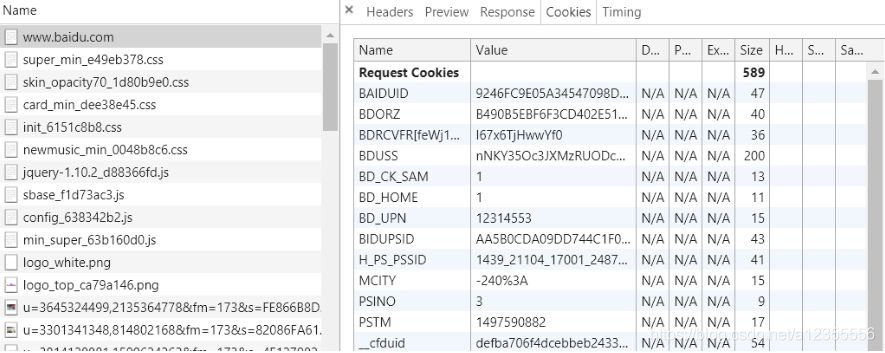
\includegraphics[width=0.80\textwidth]{img/newch1m14.png} 
\caption{Chrome 开发者工具的查看 Cookie}
\label{Test}
\end{figure}

查看 Cookie,点击 Cookies 标签可以查看在资源的 HTTP 请求和响应标头中传输的 Cookie 表。 只有传输 Cookie 时,此标签才可用。
下面是 Cookie 表中每一列的说明:

\begin{itemize}
\item [-] Name:Cookie 的名称。
\item [-] Value:Cookie 的值。
\item [-] Domain:Cookie 所属的域。
\item [-] Path:Cookie 来源的网址路径。
\item [-] Expires / Max-Age:Cookie 的 expires 或 max-age 属性的值。
\item [-] Size:Cookie 的大小 (以字节为单位)。
\item [-] HTTP:指示 Cookie 应仅由浏览器在 HTTP 请求中设置,而无法通过 JavaScript 访问。
\item [-] Secure:如果存在此属性,则指示 Cookie 应仅通过安全连接传输。
\end{itemize}

\subsection{复制、保存和清除网络信息}

右键单击 Requests Table (请求列表) 以复制、保存或删除网络信息。一些选项是上下文相关的,所以如果想在单个资源上操作,需要右键单击该资源行。下面的列表描述了每个选项。

\begin{itemize}
\item [-] Copy Response (复制响应) : 将所选资源的 HTTP 响应复制到系统剪贴板。
\item [-] Copy as cURL (复制为 cURL) : 将所选资源的网络请求作为cURL命令字符串复制到系统剪贴板。 请参阅将复制请求为 cURL 命令。 curl 命令是一个利用URL规则在命令行下工作的文件传输工具。它支持文件的上传和下载,所以是综合传输工具,但按传统,习惯称 curl 为下载工具。作为一款强力工具,curl 支持包括 HTTP、HTTPS、ftp 等众多协议,还支持 POST、cookies、认证、从指定偏移处下载部分文件、用户代理字符串、限速、文件大小、进度条等特征。做网页处理流程和数据检索自动化,curl 可以祝一臂之力。
\item [-] Copy All as HAR (全部复制为 HAR) : 将所有资源复制到系统剪贴板作为 HAR 数据。 HAR 文件包含描述网络“瀑布”的JSON数据结构。一些第三方工具可以使用HAR文件中的数据重建网络瀑布。有关详细信息,请参阅 Web 性能强大工具:HTTP 归档 (HAR)。
\item [-] Save as HAR with Content (另存为带内容的 HAR) : 将所有网络数据与每个页面资源一起保存到 HAR 文件中。 二进制资源 (包括图像) 被编码为 Base64 编码文本。
\item [-] Clear Browser Cache (清除浏览器缓存) : 清除浏览器高速缓存。当然也可以从 Network Conditions 的网络条件抽屉式窗格中启用或禁用浏览器缓存。
\item [-] Clear Browser Cookies (清除浏览器 Cookie) : 清除浏览器的 Cookie。
\item [-] Open in Sources Panel (在源文件面板中打开) : 在 Sources(源文件) 面板中打开选定的资源。
\item [-] Open Link in New Tab (在新标签页中打开链接) : 在新标签页中打开所选资源。您还可以在 Requests Table(请求列表)中双击资源名称。
\item [-] Copy Link Address (复制链接地址) : 将资源 URL 复制到系统剪贴板。
\item [-] Save (保存) : 保存所选的文本资源。仅显示在文本资源上。
\item [-] Replay XHR (重新发送 XHR) : 重新发送所选的 XMLHTTPRequest。仅显示在XHR资源上,来查看资源发起者和依赖关系,按住 Shift 并移动鼠标到资源上可查看它的发起者和依赖关系。这部分是你鼠标悬停的资源的target(目标)引用。从 target(目标)往上查找,第一个颜色编码为绿色的资源是 target(目标)的发起者。如果存在第二个颜色编码为绿色资源,那么这个是发起者的发起者。从 target(目标)向下查找,任何颜色编码为红色的资源都是 target 的依赖。
\end{itemize}

\begin{figure}[htb]
\centering 
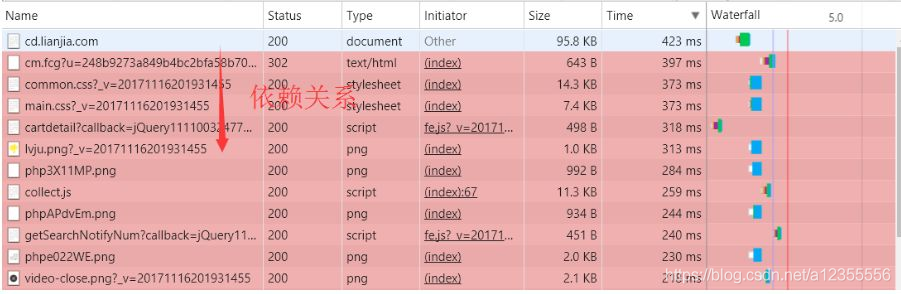
\includegraphics[width=0.80\textwidth]{img/newch1m15.png} 
\caption{Chrome 开发者工具的 Replay XHR - 重新发送 XHR}
\label{Test}
\end{figure}

\section{XAMPP 的 PHP 测试范例与凭证设定}

此节本作业除了说明 OpenSSL 等概念,也会尝试使用 XAMPP 与 PHP 分别进行凭证设定与范例,此节本作业会写程式范例同时也会提供 CA 设定档,根据写好的地区设定,在 Apache 伺服器中执行 CA 认证。

\subsection{XAMPP 说明}

XAMPP 是一个可以简单整合网页伺服器 Apache、伺服器端语言 PHP、程式语言 Perl 及资料库 MariaDB 的软体包,只要透过 XAMPP 就可以方便开发者快速架站,多数使用者在架站时需要透过网页伺服器让访客能够连到所开发的网站上,目前比较普遍的网页伺服器有简称 Apache 的 Apache HTTP 伺服器、Nginx、以及简称为 IIS 的 Microsoft Internet Information Server等,基本上透过网页伺服器就能将网页包含图像、影音等各种档案提供给请求的使用者。

PHP 最初是由勒多夫在1995年开始开发的,现在 PHP 的标准由 the PHP Group 维护,该语言是一种开源的通用计算机脚本语言,尤其适用于网络开发并可嵌入HTML中使用,其语法借鉴吸收 C 语言、 Java 和 Perl 等流行计算机语言的特点,易于一般程序员学习。而 PHP 的主要目标是允许网络开发人员快速编写动态页面,但 PHP 也被用于其他很多领域。

另外当中的 MySQL 则是在 1995 年,Michael Widenius, David Axmark 及 Allan Larsson 创立了瑞典的 MySQL AB 公司,随之推出了现今最具知名度的同名产品 MySQL,作为关联式资料库的管理所使用。所以 MySQL 从字面上来理解就是一种关联式资料库管理系统 (Relational Database Management System; RDBMS),同时也因为 MySQL 的问世,让 MySQL AB 曾经成为过去全球最大的开放源码公司。
MySQL AB 运用双重许可,一方面 MySQL 属于 GPL 的开放协议,让软体在 GPL 的规范下可以无偿使用,但这样的规范对于部分公司可能不敷使用,例如必须使用到没有被开源的程式码或技术,那就只能靠付费的方式来获得。另一方面,MySQL AB 也靠着顾问服务以及认证的方式赚取收入,例如透过开班授课、培训的方式,来取的 MySQL 的 Certificate 等方式获取利润;通过就是卖服务,MySQL可能不需要付费,但是如果要原厂支援的话则需要付费。而在 2008 年,升阳软体公司 (Sun Microsystems) 透过 10 亿美金的价格收购,而在 2009 年升阳也被甲骨文公司 (Oracle) 收购,于是乎 MySQL 成为 Oracle 旗下产品。但收购后 Oracle 大幅调涨其商业版的售价,让许多开源人士不再看好,担心有一天开源社群版最后就被会商业版取代,于是 Michael Widenius 以 MySQL 为基础,成立分支计划 MariaDB。而一些使用 MySQL 的开源专案逐渐也转向 MariaDB,例如维基百科就在 2013 年正式转换。不过因为 MariaDB 就是直接用 Fork 分流的方式从 MySQL 原始码开始开发,所以原使用者要转换到 MariaDB 上并不太困难,且外部连线函式库都可以共用。

\subsection{OpenSSL 说明}

\begin{figure}[htb]
\centering 
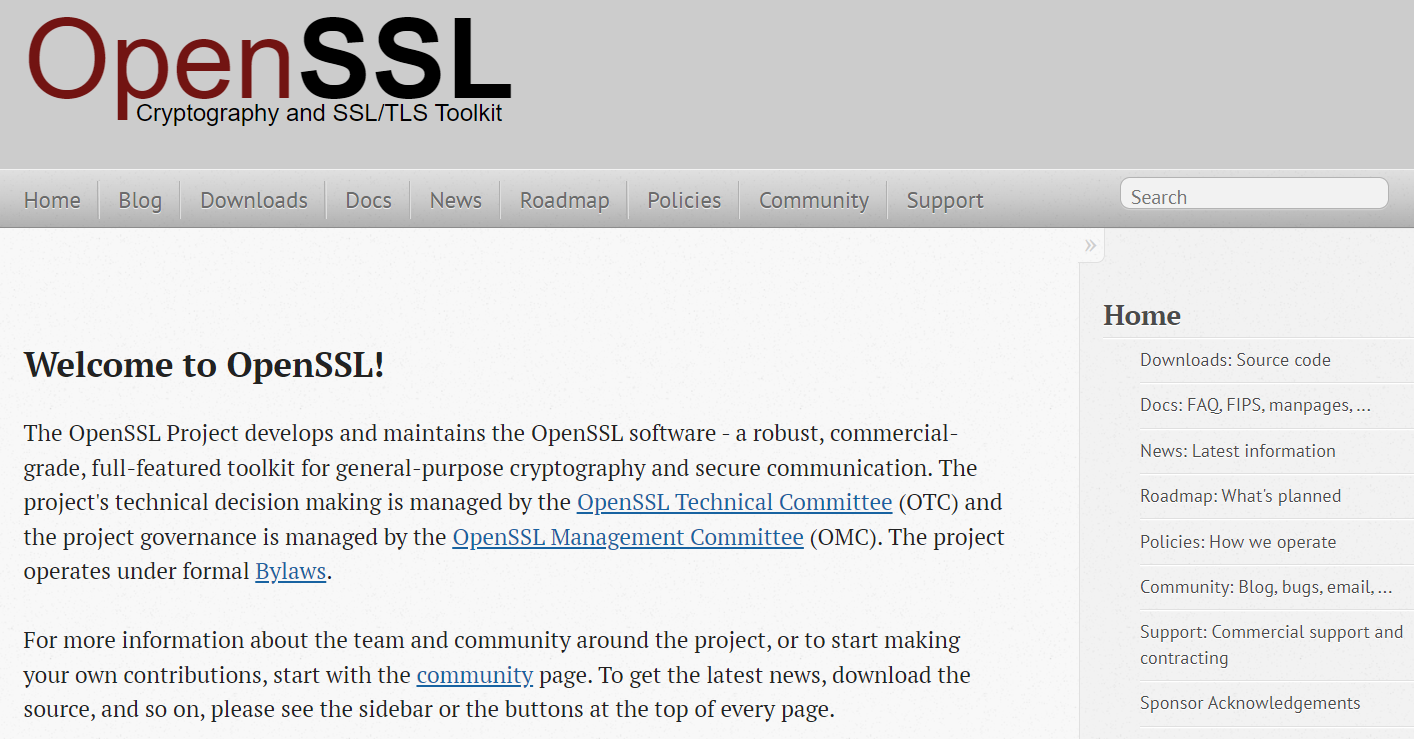
\includegraphics[width=0.80\textwidth]{img/ch1s2m1.png} 
\caption{OpenSSL 官方页面}
\label{Test}
\end{figure}

再來说明 OpenSSL,在计算机网路上 OpenSSL 是一个开放原始码的软体函式库套件,计划于 1998 年开始,该项目的目标是发明一套自由的加密工具,使之在网际网路上使用。其 OpenSSL 以 Eric Young 以及 Tim Hudson 两人所开发的 SSLeay 为基础,但随着两人前往 RSA 公司任职后, SSLeay 与 1998 年 12 月停止开发,故因此在 1998 年 12 月,社群另外分支出 OpenSSL 继续开发。目前 OpenSSL 应用程式可以使用这个套件来进行安全通讯,来避免窃听,同时确认另一端连线者的身分,此套件广泛被应用在网际网路的网页伺服器上。另外该应用的主要函式库皆是以 C 语言所写成,实作了基本的加密功能,实作了 SSL 与 TLS 协定,此外 OpenSSL 可以运行在 OpenVMS、 Microsoft Windows 以及绝大多数如 Solaris,Linux,Mac OS X 与各种版本的开放原始码 BSD 作业系统类 Unix 作业系统上。虽然此软体是开放原始码的,但其授权书条款与GPL有冲突之处,故如 Wget 等 GPL 软体使用 OpenSSL 时必须对 OpenSSL 给予例外。

\subsection{Git 说明}

Windows 的 OpenSLL 其本作业在此使用 Windows 平台版本中的 Git 内建的 OpenSSL,另外要说明的是 Git 是一个分散式版本控制软件,最初由 Linux 开发者林纳斯·托瓦兹创作,并于 2005 年以 GPL 授权条款释出,其最初目的是为了更好地管理 Linux 核心开发而设计。同时应注意的是,这与 GNU Interactive Tools 等类似 Norton Commander 界面的文件管理器有着根本上不同。 Git 最初的开发动力来自于 BitKeeper 和 Monotone,其最初只是作为一个可以被其他如 Cogito 或 Stgit 前端包装的后端而开发,但后来 Git内核已经成熟到可以独立地用作版本控制,并被很多软体专案广泛使用其中包括 Linux 核心。

\begin{figure}[htb]
\centering 
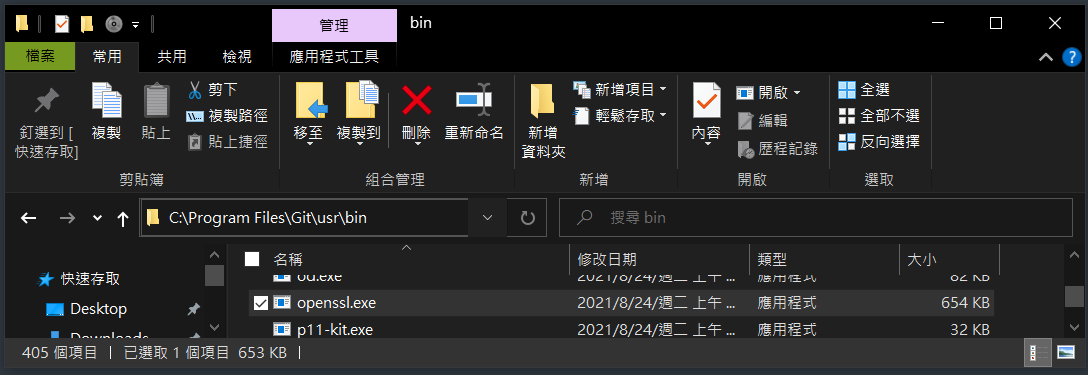
\includegraphics[width=0.80\textwidth]{img/ch1s2m2.png} 
\caption{Git 的 Windows 版本内建 OpenSSL}
\label{Test}
\end{figure}

\subsubsection{OpenSSL 的产生流程与指令结果}

在此可以看到 OpenSSL 的产生流程,但本次作业考量到便捷性故考虑使用在 Windows 的 Git 所提供的命令介面。

\begin{figure}[htb]
\centering 
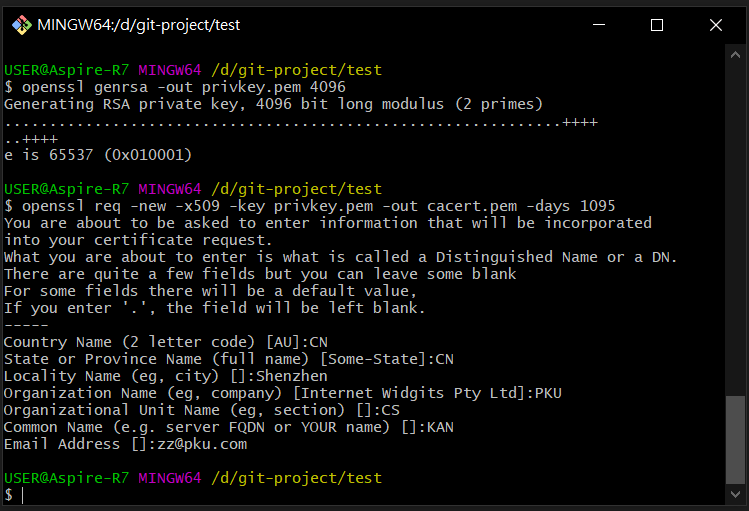
\includegraphics[width=0.80\textwidth]{img/ch1s2m3.png} 
\caption{OpenSSL 执行}
\label{Test}
\end{figure}

1. 指令

\begin{Verbatim}
openssl genrsa -out privkey.pem 4096
openssl ssh-keygen -t rsa -b 4096 -f privkey.pem
\end{Verbatim}

2. 结果

\begin{Verbatim}
USER@Aspire-R7 MINGW64 /d/git-project/test
\$ openssl genrsa -out privkey.pem 4096
Generating RSA private key, 4096 bit long modulus (2 primes)
..............................................................++++
..++++
e is 65537 (0x010001)

USER@Aspire-R7 MINGW64 /d/git-project/test
\$ openssl req -new -x509 -key privkey.pem -out cacert.pem -days 1095
You are about to be asked to enter information that will be incorporated
into your certificate request.
What you are about to enter is what is called a Distinguished Name or a DN.
There are quite a few fields but you can leave some blank
For some fields there will be a default value,
If you enter '.', the field will be left blank.
-----
Country Name (2 letter code) [AU]:CN
State or Province Name (full name) [Some-State]:CN
Locality Name (eg, city) []:Shenzhen
Organization Name (eg, company) [Internet Widgits Pty Ltd]:PKU
Organizational Unit Name (eg, section) []:CS
Common Name (e.g. server FQDN or YOUR name) []:KAN
Email Address []:zz@pku.com

USER@Aspire-R7 MINGW64 /d/git-project/test
\end{Verbatim}

\subsection{测试范例}

在此本作业为此写了 PHP 测试范例,同时也为了 APACHE 准备了设定 CA 凭证的设定档案,当中设定档案的根据皆为 XAMPP 的 APACHE 目录下。在其原目录建立 crt 目录,并放入 cert.conf 与 make-cert.bat 档案,当中 BAT 档案为 Windows 的命令档案,后者会根据前者的设定产生 CA 凭证。最后会在其 crt 目录下看到所产生的 localhost 目录。凭证设定完成后要修改其 apache \_ conf \_ extra \_ httpd-xampp.conf 档案进行设定,最后重启执行。从该目录可以看到产生的 CA 档案。另外 PHP 与 JS 档案则是根据 XAMPP 的预设目录,将其 PHP 与 HTML 档案放于 htdocs 目录下。

\subsubsection{cert.conf}

为根据 XAMPP 的 APACHE 与台湾地区所考量的 CA 设定档案。与 BAT 命令档案同放于 APACHE。

\begin{Verbatim}
[ req ]

default_bits        = 2048
default_keyfile     = server-key.pem
distinguished_name  = subject
req_extensions      = req_ext
x509_extensions     = x509_ext
string_mask         = utf8only

[ subject ]

countryName                 = Country Name (2 letter code)
countryName_default         = TW

stateOrProvinceName         = State or Province Name (full name)
stateOrProvinceName_default = Taiwan

localityName                = Locality Name (eg, city)
localityName_default        = Taipei

organizationName            = Organization Name (eg, company)
organizationName_default    = Personal Reserach

commonName                  = Common Name (e.g. server FQDN or YOUR name)
commonName_default          = localhost

emailAddress                = Email Address
emailAddress_default        = test@example.com

[ x509_ext ]

subjectKeyIdentifier   = hash
authorityKeyIdentifier = keyid,issuer

basicConstraints       = CA:FALSE
keyUsage               = digitalSignature, keyEncipherment
subjectAltName         = @alternate_names
nsComment              = "OpenSSL Generated Certificate"

[ req_ext ]

subjectKeyIdentifier = hash

basicConstraints     = CA:FALSE
keyUsage             = digitalSignature, keyEncipherment
subjectAltName       = @alternate_names
nsComment            = "OpenSSL Generated Certificate"

[ alternate_names ]

DNS.1       = localhost
\end{Verbatim}

\subsubsection{make-cert.bat}

为对应 CONF 的设定档案所设定的命令档案,在 Windows 平台上使用 PowerShell 进行执行,最后产生 CA 档案。

\begin{Verbatim}
@echo off
::set /p domain="Enter Domain: "
set domain="localhost"
set OPENSSL_CONF=../conf/openssl.cnf

if not exist .\%domain\% mkdir .\%domain\%

..\bin\openssl req -config cert.conf -new -sha256 -newkey rsa:2048 -nodes -keyout\
\%domain\%\server.key -x509 -days 3650 -out \%domain\%\server.crt

echo.
echo -----
echo The certificate was provided.
echo.
\end{Verbatim}

\subsubsection{http-s-index.php}

为测试 HTTP 和 HTTPS 所特地准备的档案,当中的 PHP 根据路径与资讯进行判断。

\begin{Verbatim}
<!DOCTYPE html>
<html>
<head>
	<meta charset="utf-8">
	<meta name="viewport" content="width=device-width, initial-scale=1">
	<title>TEST - HTTP & HTTPS</title>
	<style type="text/css">
		body {
			text-align: center;
		}
	</style>
</head>
<body>
	<h1>TEST - HTTP & HTTPS</h1>
	<div>
		<?php
			if (!empty($_SERVER['HTTPS']) && ('on' == $_SERVER['HTTPS'])) {
				$uri = 'https://';
				echo "目前是 HTTPS";
			} else {
				$uri = 'http://';
				echo "目前是 HTTP";
			}
			$uri .= $_SERVER['HTTP_HOST'];
			phpinfo();
		?>	
	</div>
</body>
</html>
\end{Verbatim}

\subsubsection{http-s-index.html}

为测试 HTTP 和 HTTPS 所特地准备的档案,当中的 JS 根据路径与资讯进行判断。

\begin{Verbatim}
<!DOCTYPE html>
<html>
<head>
	<meta charset="utf-8">
	<meta name="viewport" content="width=device-width, initial-scale=1">
	<title>TEST - HTTP & HTTPS</title>
	<style type="text/css">
		body {
			text-align: center;
		}
	</style>
</head>
<body>
	<h1>TEST - HTTP & HTTPS</h1>
	<div>
		<span id="show"></span>
	</div>
</body>
<script type="text/javascript">
	var ishttps = 'https:' == document.location.protocol ? true: false;
	if(ishttps){
		// alert("这是一个 HTTPS 请求");
		document.getElementById("show").textContent="这是一个 HTTPS 请求";
	}else{
		// alert("这是一个 HTTP 请求");
		document.getElementById("show").textContent="这是一个 HTTP 请求";
	}
</script>
</html>
\end{Verbatim}

\subsubsection{httpd-xampp.conf}

安装完凭证后,需要在 APACHE 对 httpd-xampp.conf 进行设定,最后重启 APACHE。

\begin{Verbatim}
## localhost
<VirtualHost *:80>
    DocumentRoot "C:/xampp/htdocs"
    ServerName localhost

    ServerAlias *.localhost

   RewriteEngine On
    RewriteCond \%{HTTPS} off
   RewriteRule (.*) https://\%{SERVER_NAME}/\$1 [R,L]
</VirtualHost>
<VirtualHost *:443>
    DocumentRoot "C:/xampp/htdocs"
    ServerName localhost

    ServerAlias *.localhost
   SSLEngine on
   SSLCertificateFile "crt/localhost/server.crt"
   SSLCertificateKeyFile "crt/localhost/server.key"
</VirtualHost>
\end{Verbatim}

\subsection{PHP 的 Web Server 方案}

此外本作业针对 XAMPP,同时也准备了备案,其 PHP 内建有 Web Server 的方案,其作用是提供使用者一个方便的测试用途。本作业根据此作为测试的备案。从 PHP 的指令中可以看到,其参数为大写的 S,最后加上 IP 位址与 Port 号。

1. 指令

\begin{Verbatim}
> php -S 127.0.0.1:9988
\end{Verbatim}

2. PHP 帮助

\begin{Verbatim}
Usage: php [options] [-f] <file> [--] [args...]
   php [options] -r <code> [--] [args...]
   php [options] [-B <begin_code>] -R <code> [-E <end_code>] [--] [args...]
   php [options] [-B <begin_code>] -F <file> [-E <end_code>] [--] [args...]
   php [options] -S <addr>:<port> [-t docroot] [router]
   php [options] -- [args...]
   php [options] -a

  -a               Run as interactive shell
  -c <path>|<file> Look for php.ini file in this directory
  -n               No configuration (ini) files will be used
  -d foo[=bar]     Define INI entry foo with value 'bar'
  -e               Generate extended information for debugger/profiler
  -f <file>        Parse and execute <file>.
  -h               This help
  -i               PHP information
  -l               Syntax check only (lint)
  -m               Show compiled in modules
  -r <code>        Run PHP <code> without using script tags <?..?>
  -B <begin_code>  Run PHP <begin_code> before processing input lines
  -R <code>        Run PHP <code> for every input line
  -F <file>        Parse and execute <file> for every input line
  -E <end_code>    Run PHP <end_code> after processing all input lines
  -H               Hide any passed arguments from external tools.
  -S <addr>:<port> Run with built-in web server.
  -t <docroot>     Specify document root <docroot> for built-in web server.
  -s               Output HTML syntax highlighted source.
  -v               Version number
  -w               Output source with stripped comments and whitespace.
  -z <file>        Load Zend extension <file>.

  args...          Arguments passed to script. Use -- args when first argument
                   starts with - or script is read from stdin

  --ini            Show configuration file names

  --rf <name>      Show information about function <name>.
  --rc <name>      Show information about class <name>.
  --re <name>      Show information about extension <name>.
  --rz <name>      Show information about Zend extension <name>.
  --ri <name>      Show configuration for extension <name>.
\end{Verbatim}

\subsection{凭证设定}

根据本作业前几个小节,可以知道其事前工作的准备。同时可以看到此小节执行 BAT 与 APACHE 产生凭证后,对其进行安装,最后于 Windows 平台检视其结果。同时也看到测试范例显示的资讯。


\begin{figure}[htb]
\centering 
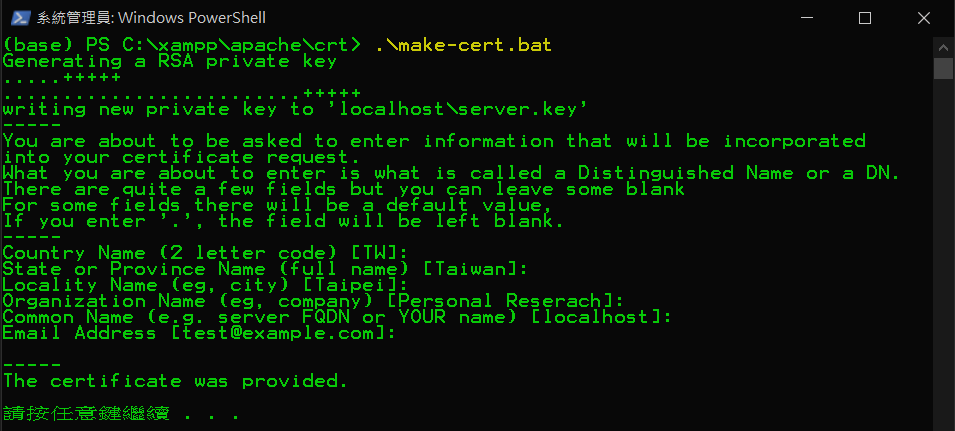
\includegraphics[width=0.80\textwidth]{img/ch1s2m4.png} 
\caption{执行 BAT 范例}
\label{Test}
\end{figure}

\begin{figure}[htb]
\centering 
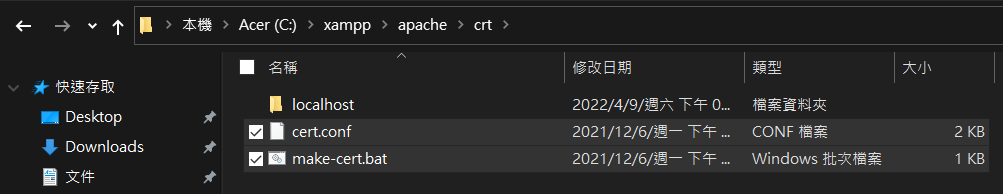
\includegraphics[width=0.80\textwidth]{img/ch1s2m5.png} 
\caption{APACHE 结果}
\label{Test}
\end{figure}

\begin{figure}[htb]
\centering 
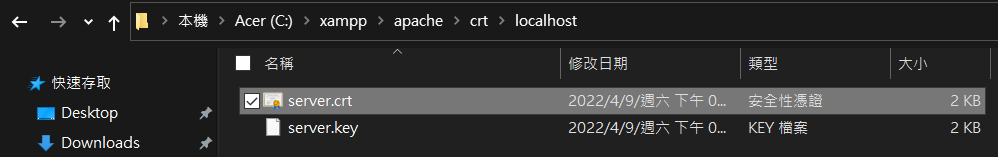
\includegraphics[width=0.80\textwidth]{img/ch1s2m6.png} 
\caption{证书}
\label{Test}
\end{figure}

\begin{figure}[htb]
\centering 
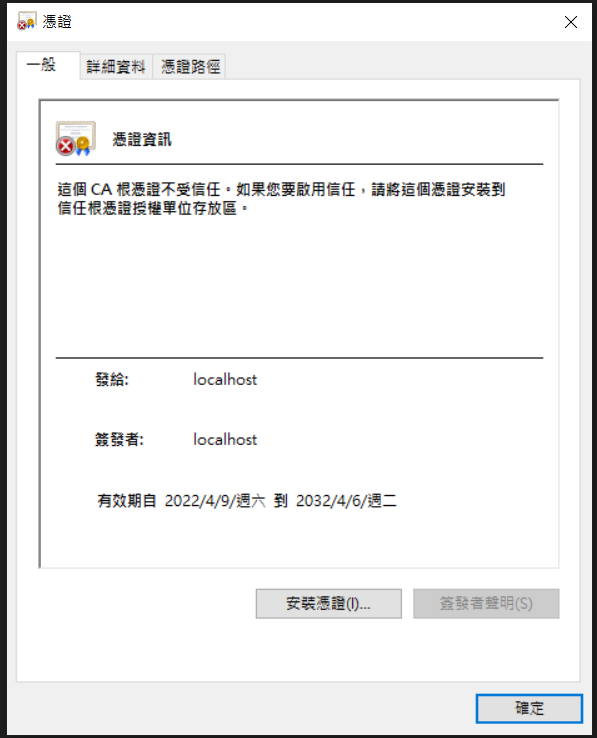
\includegraphics[width=0.80\textwidth]{img/ch1s2m7.png} 
\caption{安装证书}
\label{Test}
\end{figure}

\begin{figure}[htb]
\centering 
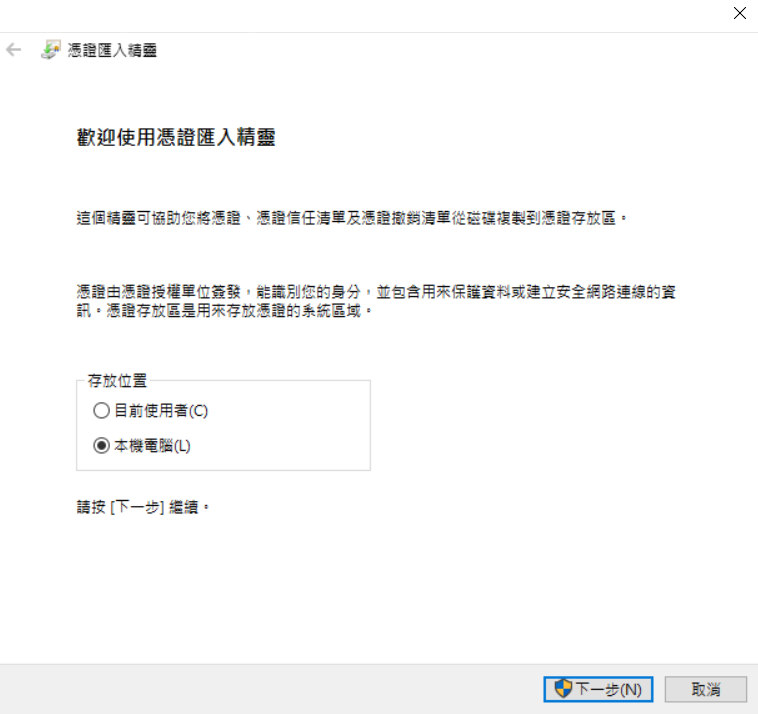
\includegraphics[width=0.80\textwidth]{img/ch1s2m8.png} 
\caption{汇入流程}
\label{Test}
\end{figure}

\begin{figure}[htb]
\centering 
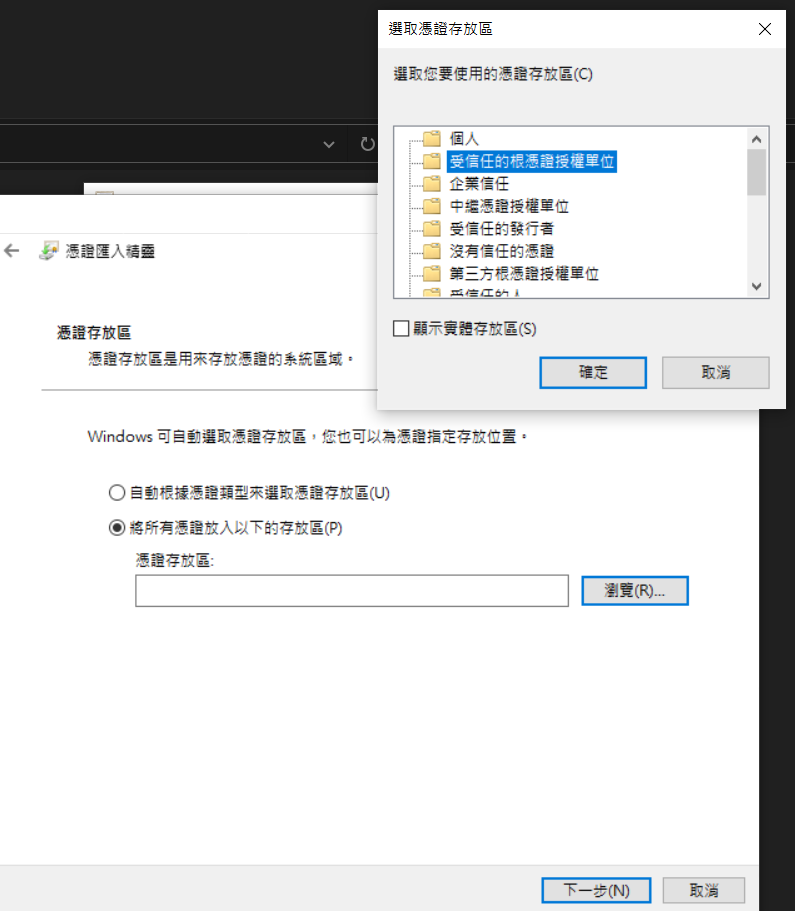
\includegraphics[width=0.80\textwidth]{img/ch1s2m9.png} 
\caption{受信任的跟凭证授权单位}
\label{Test}
\end{figure}

\begin{figure}[htb]
\centering 
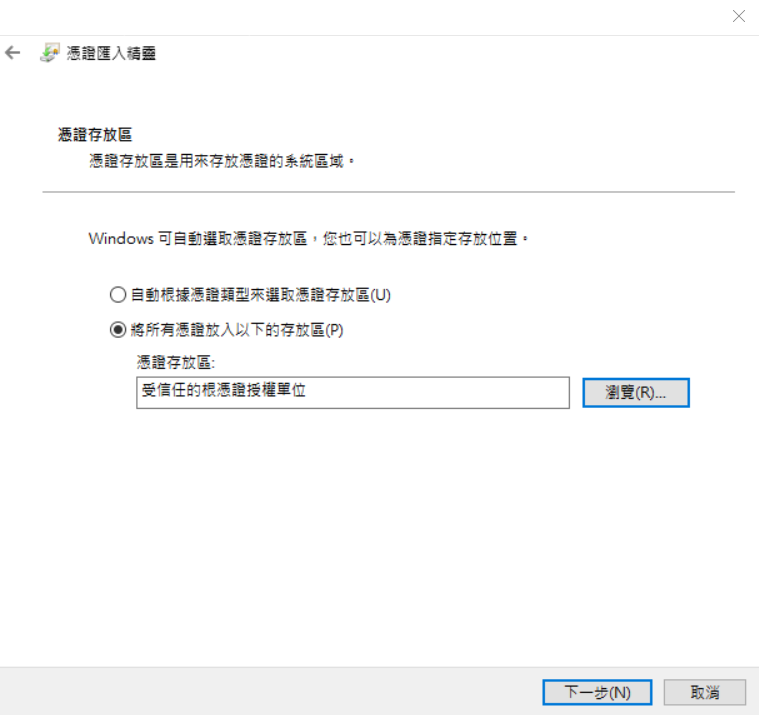
\includegraphics[width=0.80\textwidth]{img/ch1s2m10.png} 
\caption{设定存放}
\label{Test}
\end{figure}

\begin{figure}[htb]
\centering 
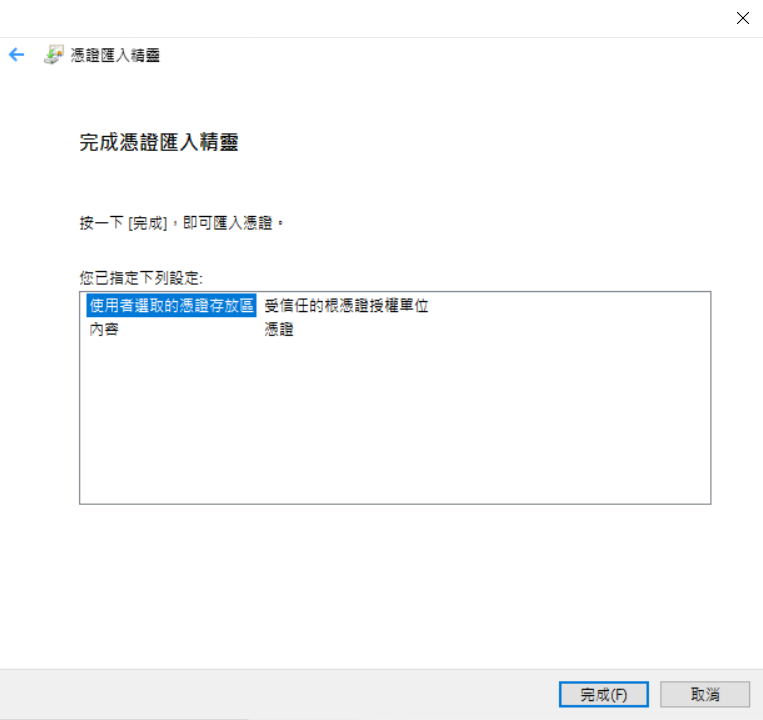
\includegraphics[width=0.80\textwidth]{img/ch1s2m11.png} 
\caption{完成凭证}
\label{Test}
\end{figure}

\begin{figure}[htb]
\centering 
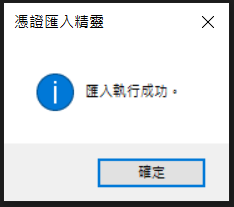
\includegraphics[width=0.40\textwidth]{img/ch1s2m12.png} 
\caption{确定凭证}
\label{Test}
\end{figure}

\begin{figure}[htb]
\centering 
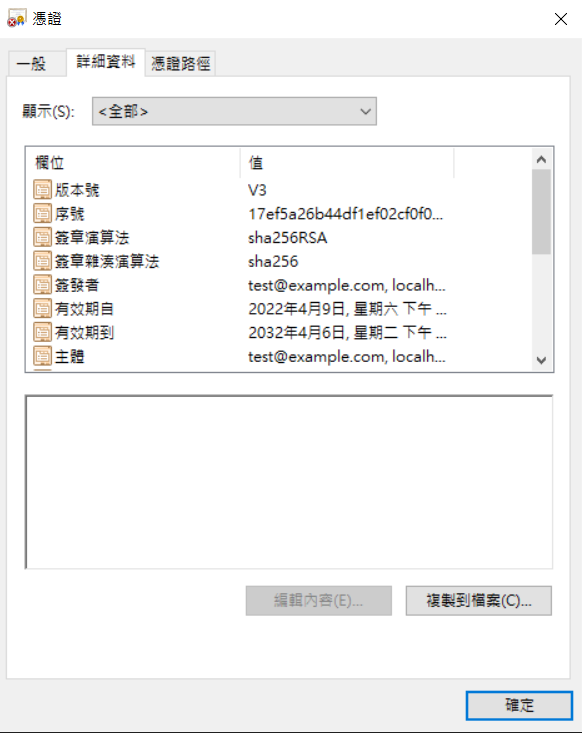
\includegraphics[width=0.70\textwidth]{img/ch1s2m13.png} 
\caption{检视凭证资讯}
\label{Test}
\end{figure}

\begin{figure}[htb]
\centering 
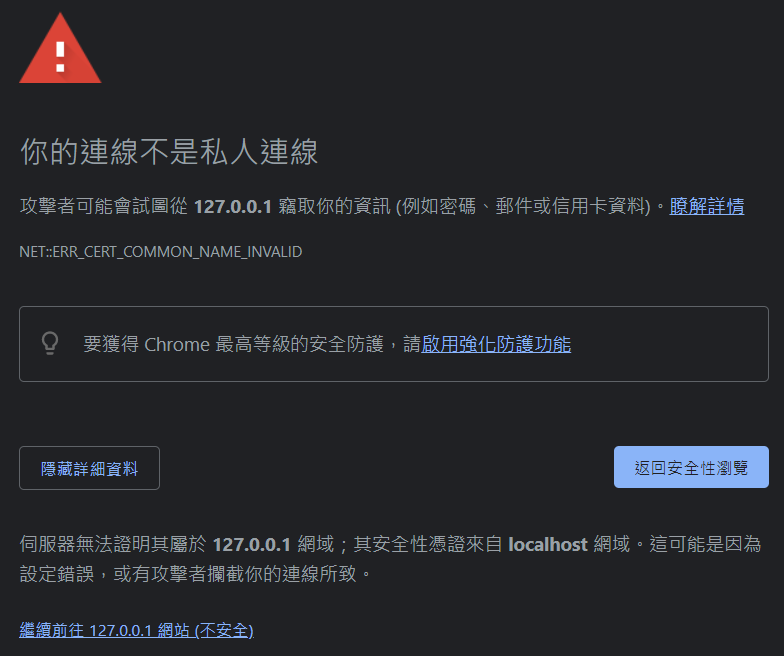
\includegraphics[width=0.70\textwidth]{img/ch1s2m14.png} 
\caption{执行画面}
\label{Test}
\end{figure}

\begin{figure}[htb]
\centering 
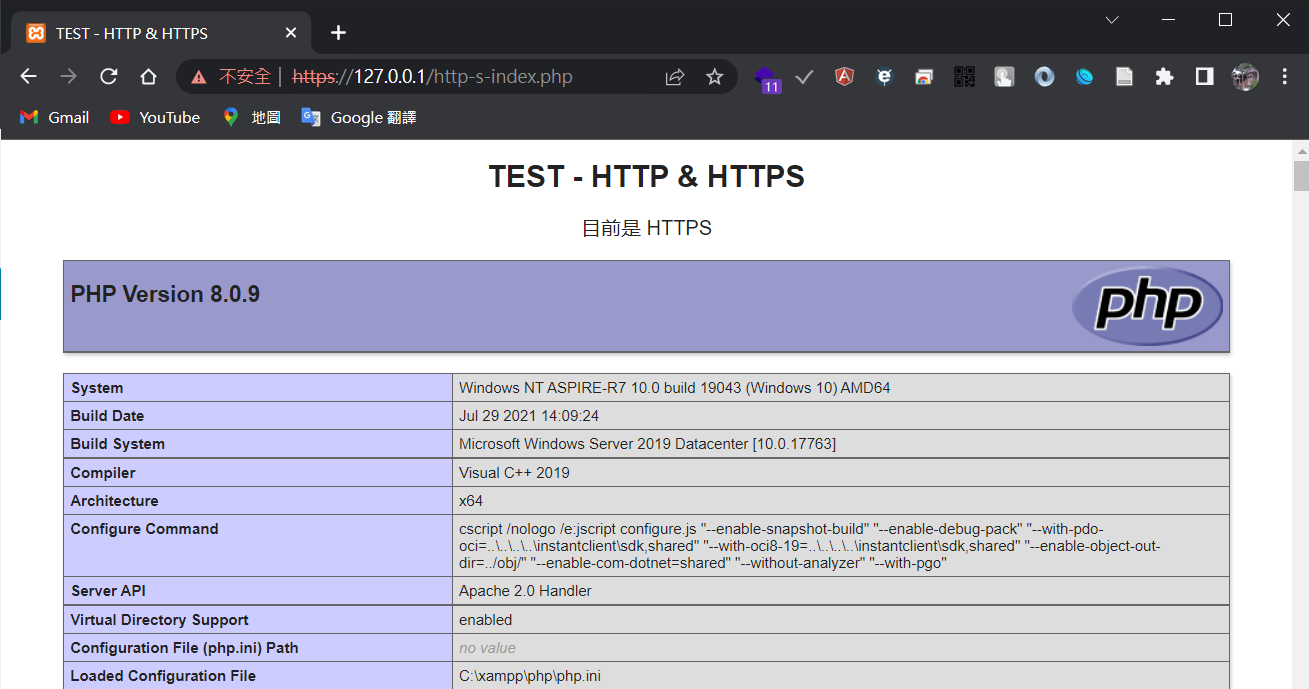
\includegraphics[width=0.70\textwidth]{img/ch1s2m15.png} 
\caption{PHP 版本}
\label{Test}
\end{figure}

\begin{figure}[htb]
\centering 
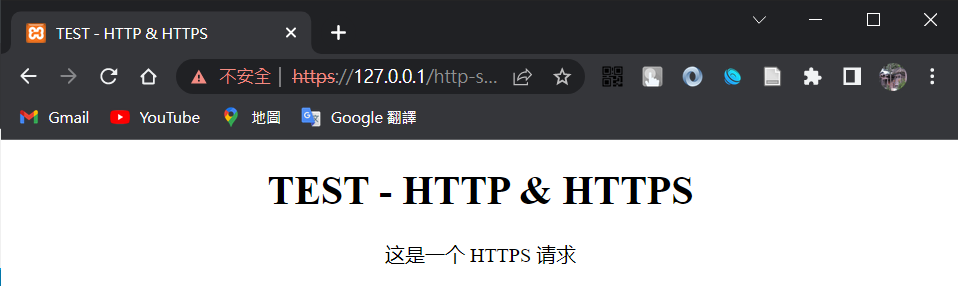
\includegraphics[width=0.70\textwidth]{img/ch1s2m16.png} 
\caption{JS 版本}
\label{Test}
\end{figure}


\section{移除凭证}

本节接续前一小节说明在 Windows 平台安装后的凭证移除,首先找 MMC,进入主控台进行移除的设定,同时将凭证选项加入管理,同时设定帐户的权限范围,最后对成功的证书进行移除,移除成功后根据上一节的状况,要将 APACHE 的设定移掉,最后重启 APACHE。

\begin{figure}[htb]
\centering 
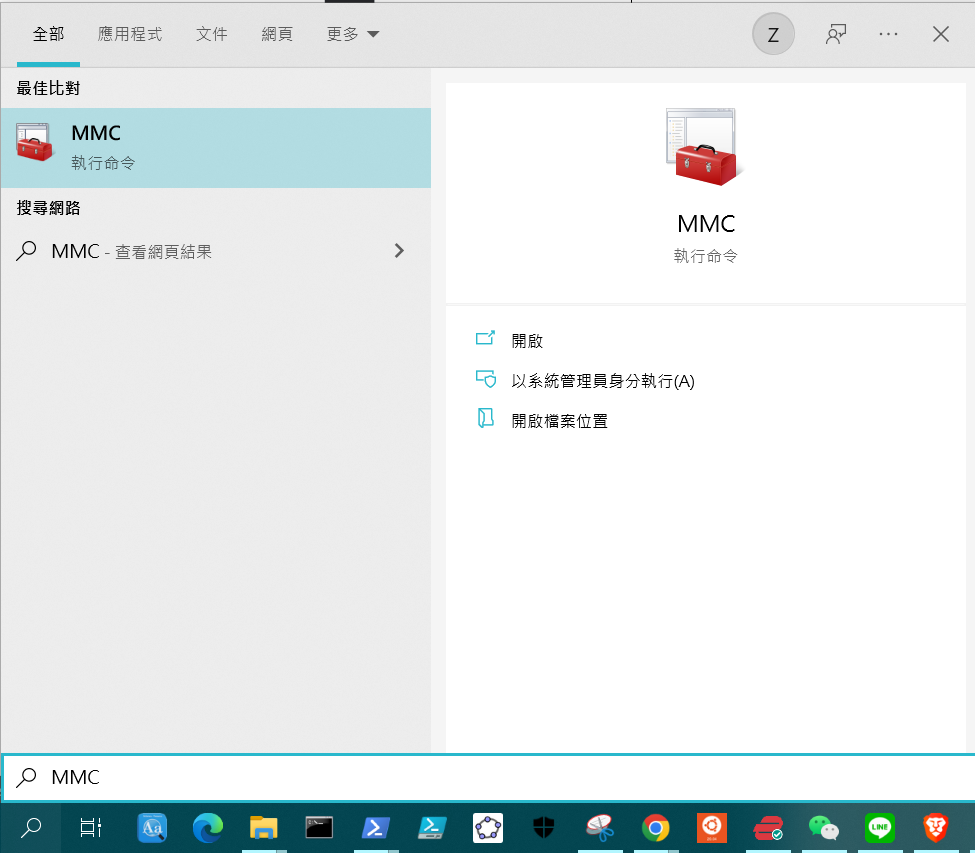
\includegraphics[width=0.70\textwidth]{img/ch1s3m1.png} 
\caption{找 MMC}
\label{Test}
\end{figure}

\begin{figure}[htb]
\centering 
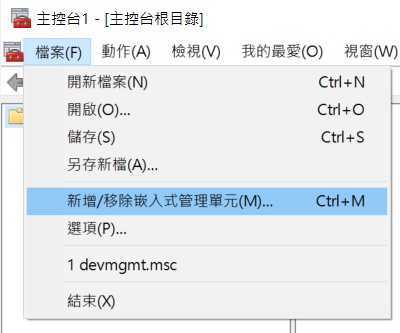
\includegraphics[width=0.50\textwidth]{img/ch1s3m2.png} 
\caption{主控台移除}
\label{Test}
\end{figure}

\begin{figure}[htb]
\centering 
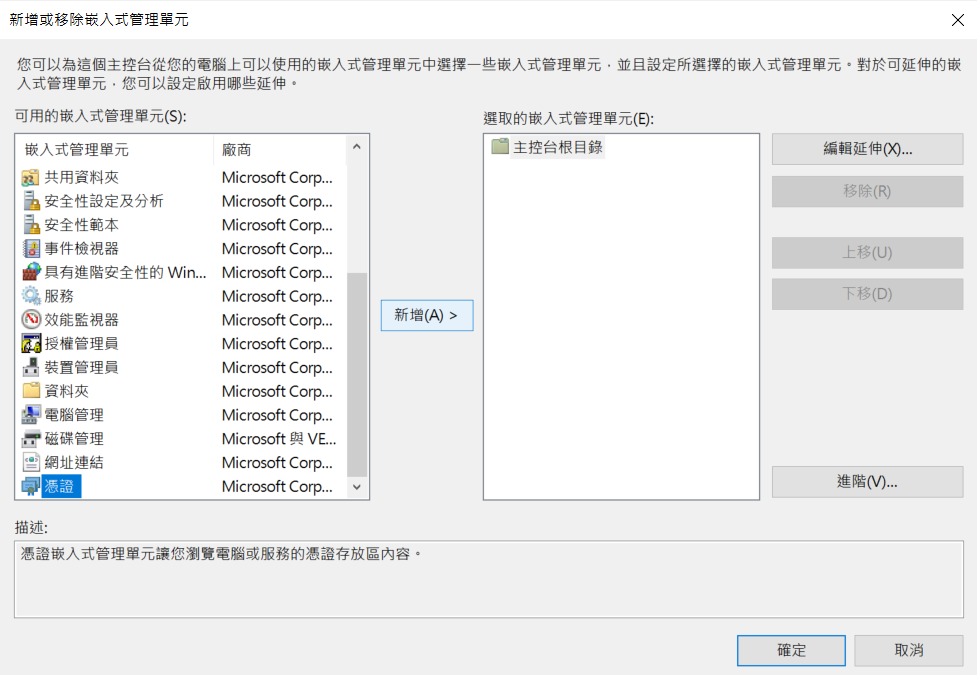
\includegraphics[width=0.70\textwidth]{img/ch1s3m3.png} 
\caption{将凭证加入管理}
\label{Test}
\end{figure}

\begin{figure}[htb]
\centering 
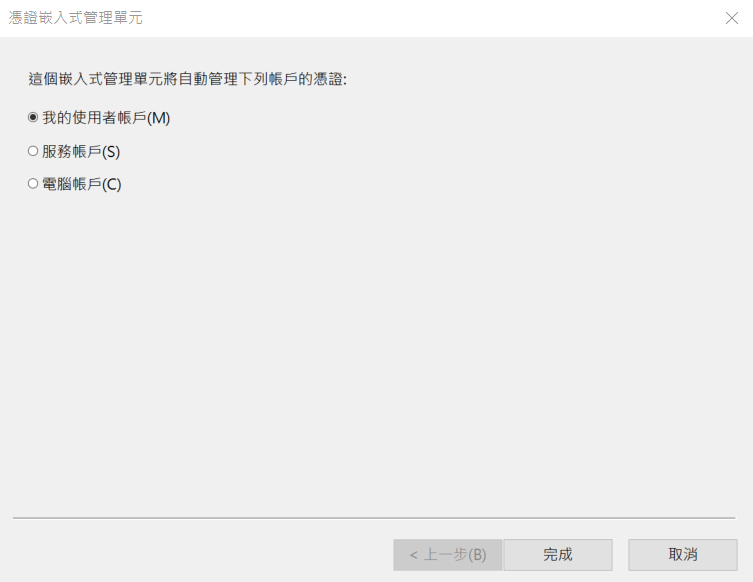
\includegraphics[width=0.70\textwidth]{img/ch1s3m4.png} 
\caption{设定帐户}
\label{Test}
\end{figure}

\begin{figure}[htb]
\centering 
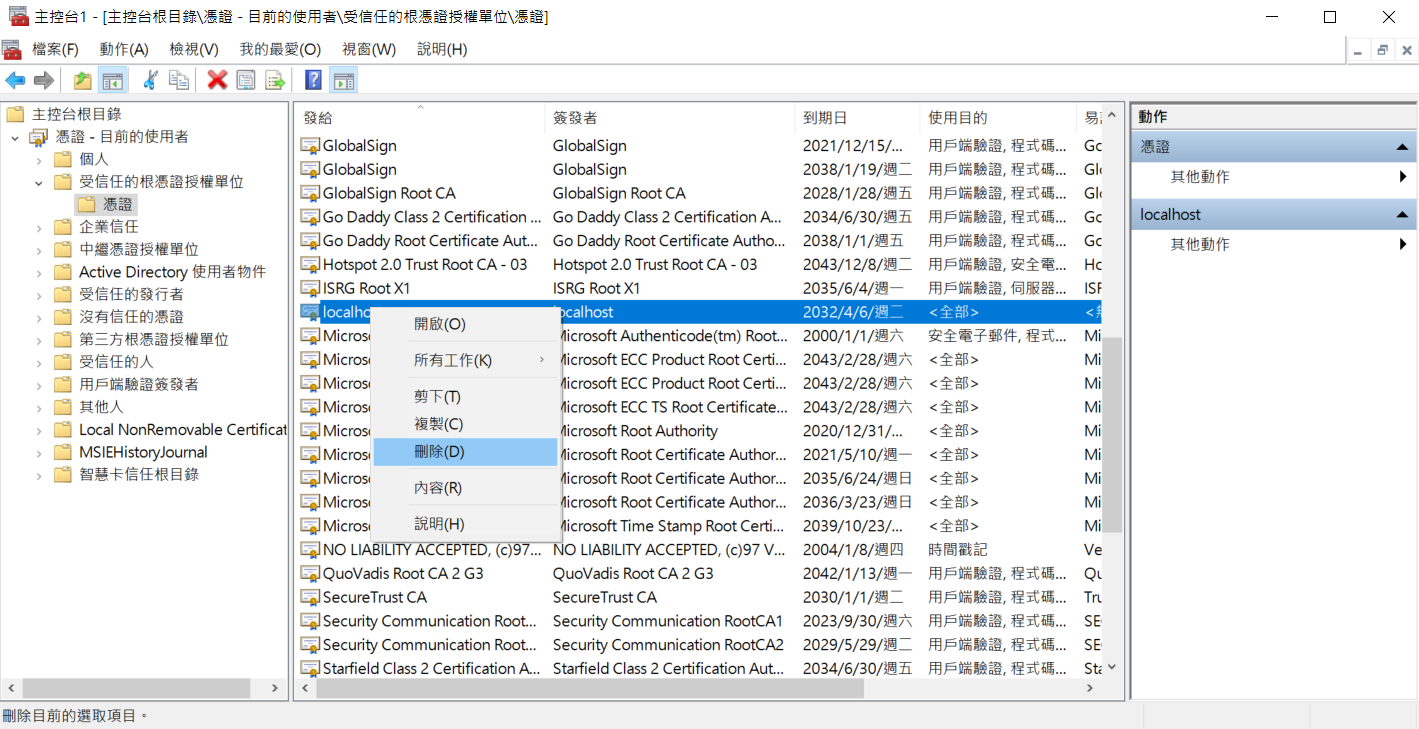
\includegraphics[width=0.70\textwidth]{img/ch1s3m5.png} 
\caption{移除}
\label{Test}
\end{figure}

\section{进行 HTTP 与 HTTPS 分析}

本作业此节使用 Mac 的 Wireshark,对 HTTPS 与 HTTP 两个现有的网路服务进行分析,同时使用 Mac 平台的 Wireshark 工具进行判断与分析,从结果来说,很明显得可以从各自的 TCP 串流中可以看到安全性问题。

\begin{figure}[htb]
\centering 
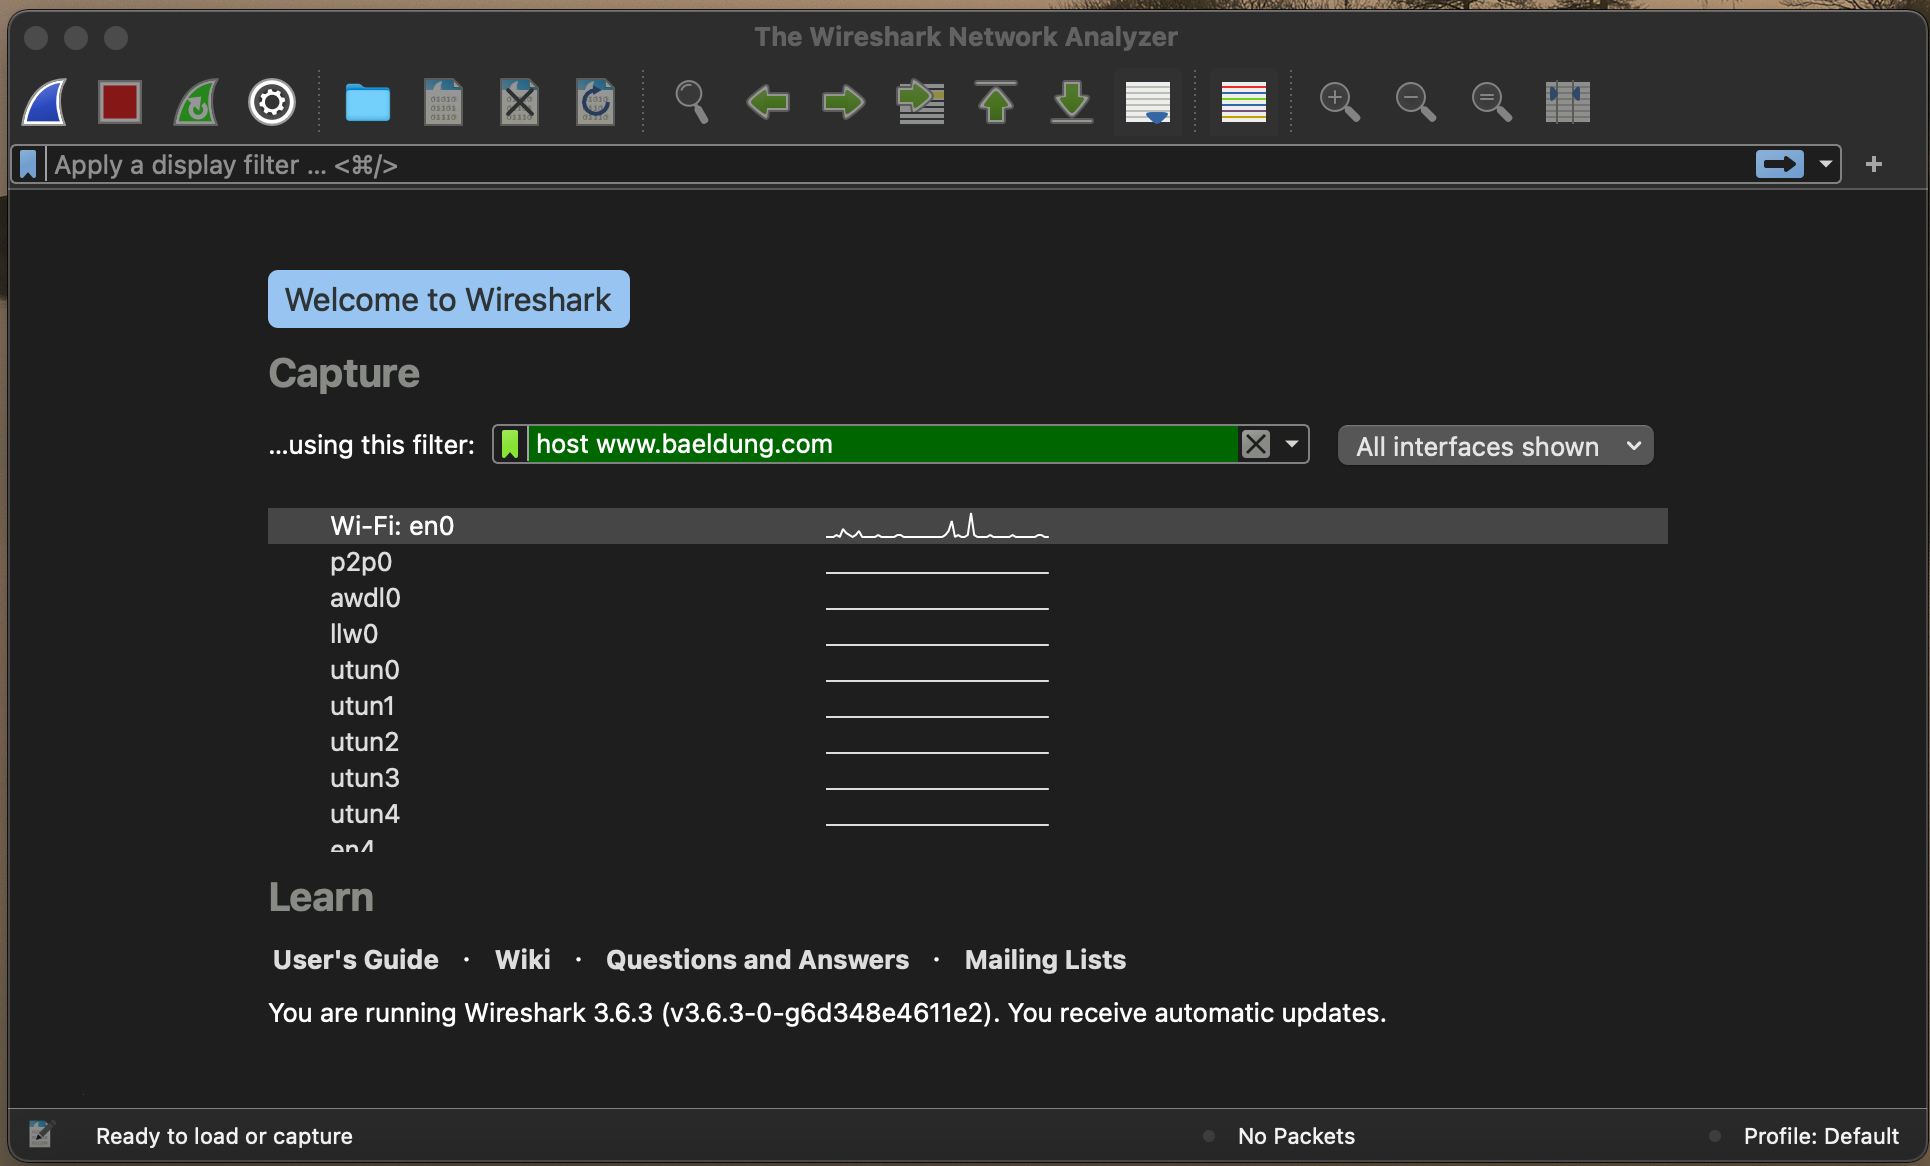
\includegraphics[width=0.70\textwidth]{img/ch1s4m1.png} 
\caption{Mac 的 Wireshark}
\label{Test}
\end{figure}

\begin{figure}[htb]
\centering 
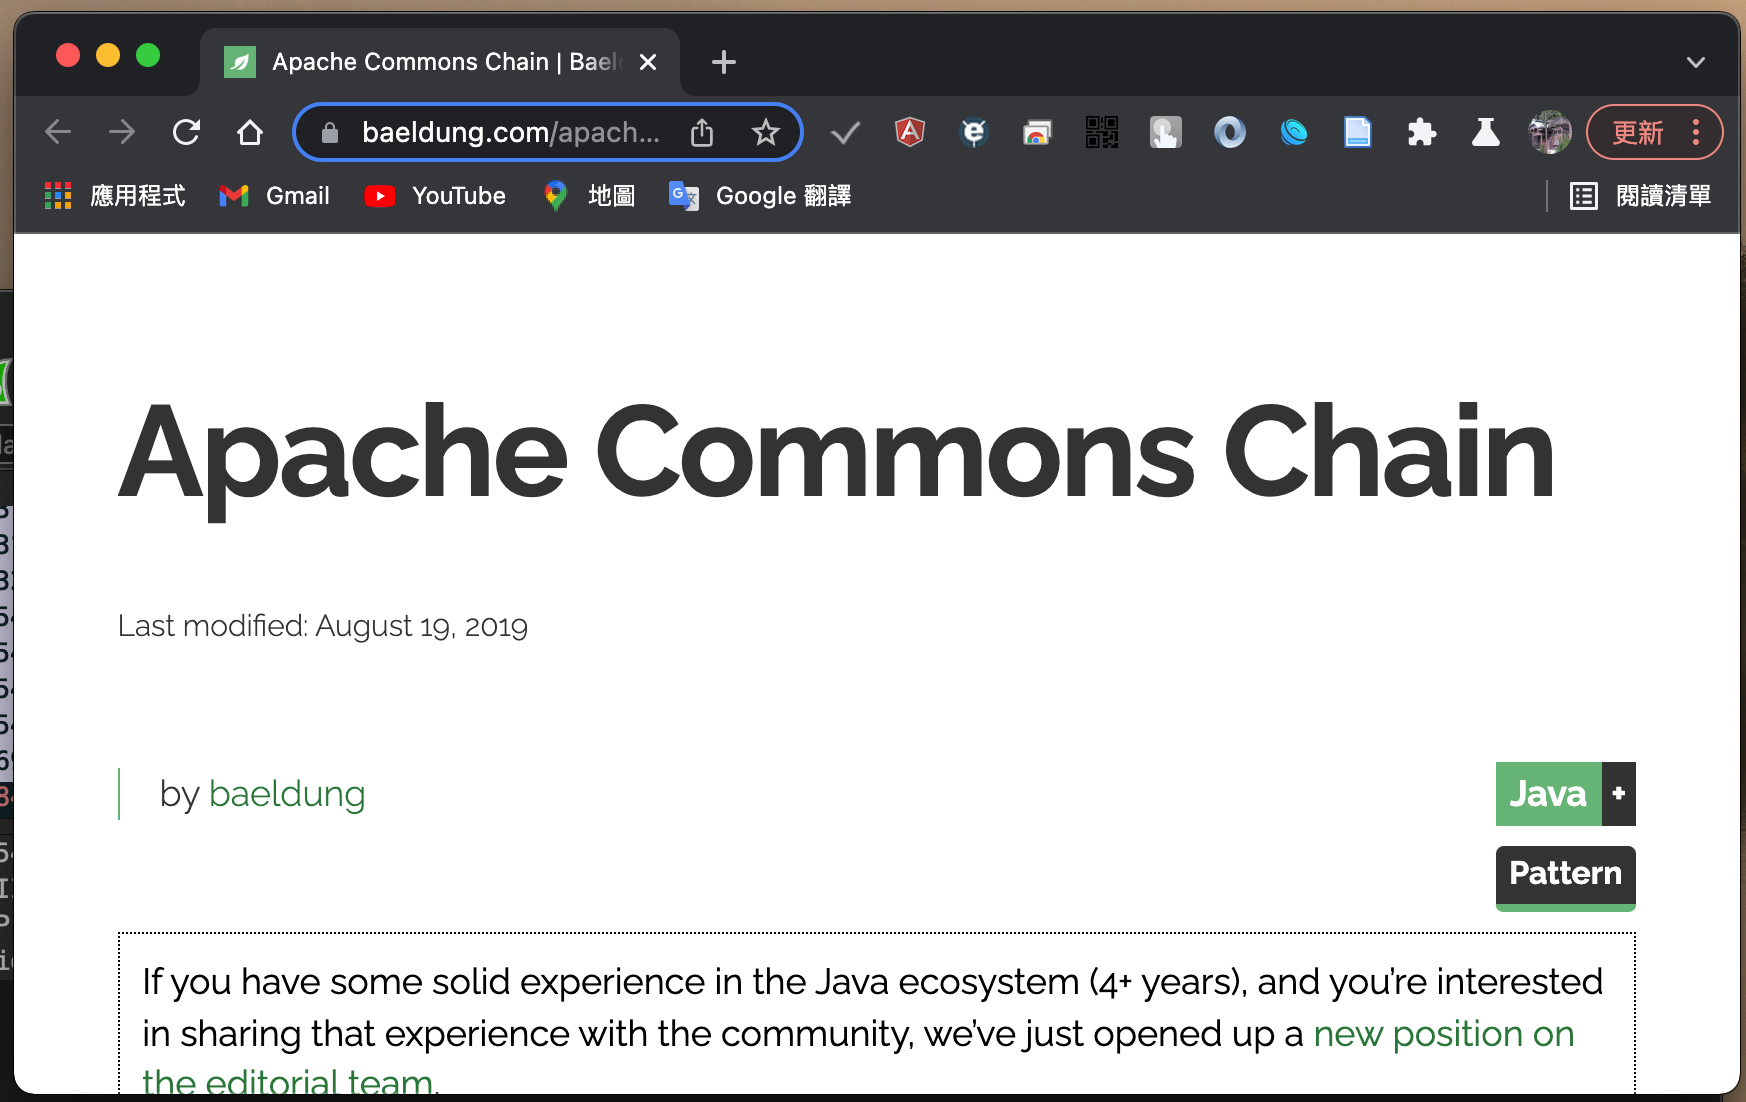
\includegraphics[width=0.70\textwidth]{img/ch1s4m2.png} 
\caption{HTTPS 服务范例}
\label{Test}
\end{figure}

\begin{figure}[htb]
\centering 
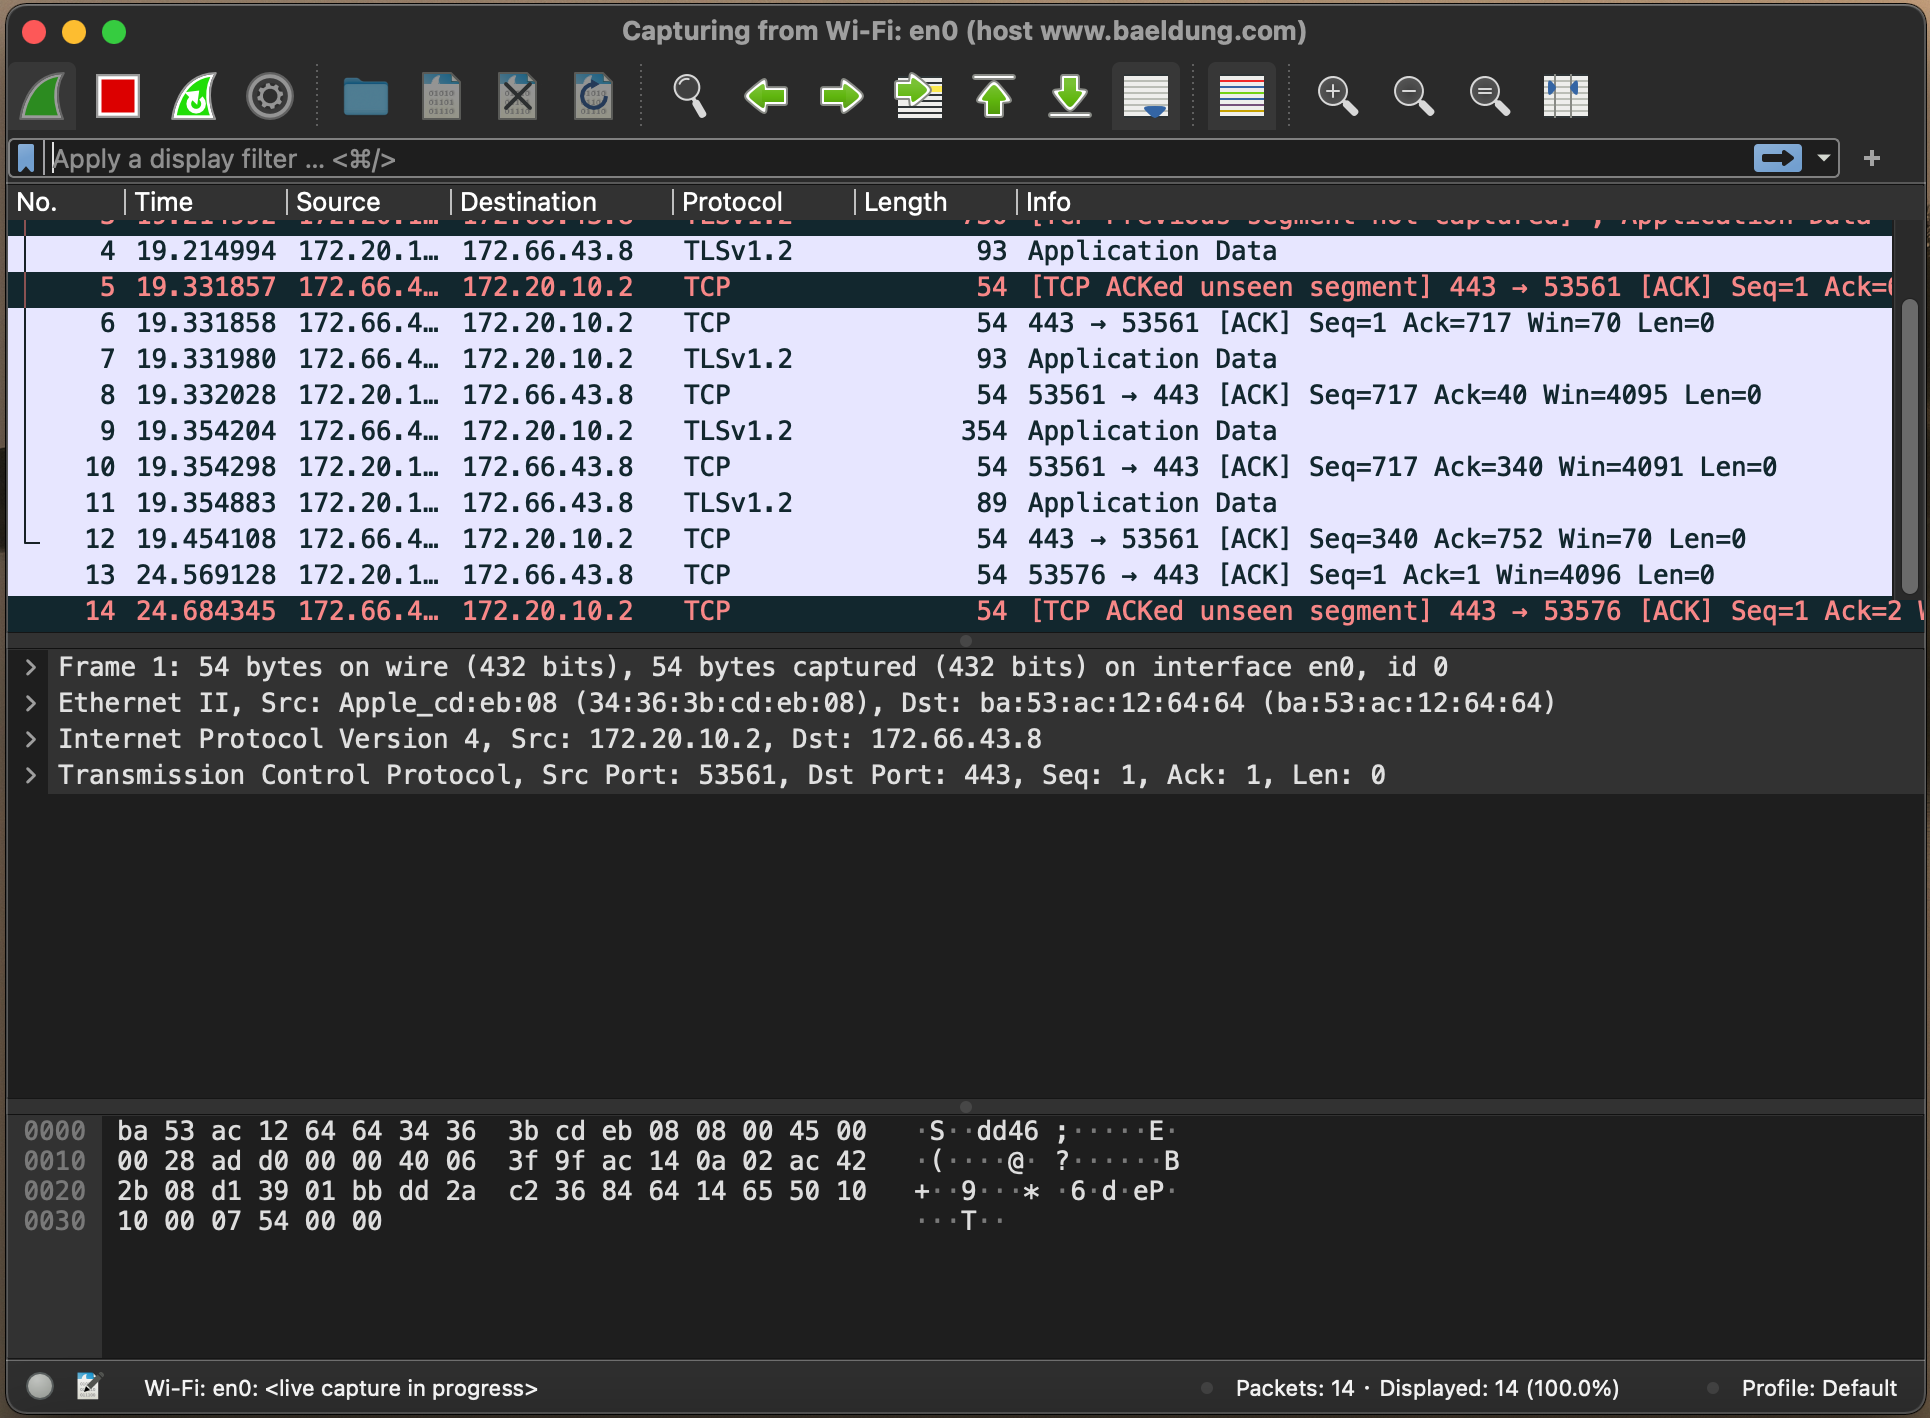
\includegraphics[width=0.70\textwidth]{img/ch1s4m3.png} 
\caption{Wireshark 判断 HTTPS}
\label{Test}
\end{figure}

\begin{figure}[htb]
\centering 
\includegraphics[width=0.70\textwidth]{img/ch1s4m4.png} 
\caption{找 TCP 串流}
\label{Test}
\end{figure}

\begin{figure}[htb]
\centering 
\includegraphics[width=0.70\textwidth]{img/ch1s4m5.png} 
\caption{HTTPS 结果}
\label{Test}
\end{figure}

\begin{figure}[htb]
\centering 
\includegraphics[width=0.70\textwidth]{img/ch1s4m6.png} 
\caption{测试 HTTP}
\label{Test}
\end{figure}

\begin{figure}[htb]
\centering 
\includegraphics[width=0.70\textwidth]{img/ch1s4m7.png} 
\caption{Wireshark 判断 HTTP}
\label{Test}
\end{figure}

\begin{figure}[htb]
\centering 
\includegraphics[width=0.70\textwidth]{img/ch1s4m8.png} 
\caption{HTTP 结果}
\label{Test}
\end{figure}

\begin{figure}[htb]
\centering 
\includegraphics[width=0.70\textwidth]{img/ch1s4m9.png} 
\caption{HTTP 服务范例}
\label{Test}
\end{figure}


\section{WiFi 探针原理与说明}

\subsection{何为 WiFi 探针}

所谓的 WiFi 探针技术是根据 WiFi 探测技术来识别用途名为 AP 的无线访问接入点,附近已开启 WiFi 的智能手机或者类似于笔记本,平板电脑等 WiFi终端,其无需使用者接入 WiFi,WiFi 探针就能够识别使用者的信息。而当使用者走进探针信号覆盖区域内且使用者的 WiFi 设备开启时,其的设备就能被探针探测并发现,所以无论是 Apple 的 IOS 或者是 Google 安卓系统都能轻易检测,并且获取设备的 MAC 地址与相关资讯。其特点如下所示:

\begin{itemize}
\item [-] 用户无需参与,无需连接到网络
\item [-] Android , IOS 全兼容
\item [-] 自动探测区域内手机 MAC 地址
\item [-] 手机,平板均能探测
\end{itemize}

\subsection{工作原理}

WiFi 是基于 IEEE 802.11a/b/g/n 协议而成,在标准协议中,定义了名为 AP 的无线接入点和名为站或客户端的 STA 的两种工作模式,同时协议中规定了 BEACON、ACK、DATA、PROBE 等多种无线数据帧类型,在站连接到无线接入点时进行交互的就是数据桢和应答帧、同时 AP 周期性发送BEACON。在站点没有连接到无线接入点上,手机客户端等站点也会发送 PROBE 帧进行探测询问哪个 AP 是可以连接使用。其 WiFi 探针就是基于各种无线数据帧来抓获手机等 WIFI 客户端的 MAC 地址信息。每个 AP 每隔几十毫秒到几秒不等一定时间会向周围的 STA 和 A P广播 BEACON 帧,就是告诉周围的 STA 和其他的 AP,自己是 xxxx 的 bssid,发出快来连接我的请求,同时每个 STA,如手机、笔记本等除了默默监听周边 AP 发送的 BEACON 帧以外,还会偷偷发送 PROBE 帧,类似于 我是 xxxx 的 MAC 地址,我能够连结的请求。

\subsection{深入了解}

要深入了解 WiFi 探针技术,首先先认识 WiFi 所使用的网络协议,WiFi采用的是IEEE802.11协议集,此协议集包含许多子协议。其中按照时间顺序发展,主要有:(1) 802.11a,(2) 802.11b, (3) 802.11g,(4) 802.11n。同时在网络通信中,数据被封装成了帧,而帧就是指通信中的一个数据块。但是帧在数据链路层传输的时候是有固定格式的,不是随意的封装和打包就可以传输,大小有限制,最小 46 字节,最大 1500 字节,所以必须按照此规则来封装。下面为 802.11 的帧结构,且从上面的结构可以知道,前俩个字节为:帧控制字段,控制字段的前 2 BIT 节为协议类型,且目前此值为:0。

\begin{figure}[htb]
\centering 
\includegraphics[width=0.70\textwidth]{img/ch1s5m1.jpg} 
\caption{802.11 的帧}
\label{Test}
\end{figure}

\begin{figure}[htb]
\centering 
\includegraphics[width=0.70\textwidth]{img/ch1s5m2.jpg} 
\caption{帧控制字段}
\label{Test}
\end{figure}

\begin{itemize}
\item [-] 控制帧 (Control Frame) : 如 RTS 帧、CTS 帧、 ACK 帧用于竞争期间的握手通信和正向确认、结束非竞争期等。
\item [-] 管理帧 (Management Frame) : 如 Beacon 帧、Probe Request 帧,主要用于 STA 与 AP 之间协商、关系的控制,而控制行为如关联、认证、同步等。
\item [-] 数据帧 (Data Frame) : 为承载数据的载体,用于在竞争期和非竞争期传输数据。
\end{itemize}

\subsubsection{信标帧}

信标帧 (BeaconFrame) 是相当重要的维护机制,主要来宣告某个 AP 网络的存在,同时会定期发送的信标,可让移动 WiFi 设备得知该网络的存在,从而调整加入该网络所必要的参数。而在基础网络里,AP 必须负责发送 Beacon 帧,而 Beacon帧的所及范围即为基本服务区域。同时在基础型网络里,所有沟通都必须通过接入点,因此 WiFi 设备不能距离太远,否则无法接收到信标。下图可以看到帧格式的说明。

\begin{figure}[htb]
\centering 
\includegraphics[width=0.70\textwidth]{img/ch1s5m3.jpg} 
\caption{信标帧}
\label{Test}
\end{figure}


\subsubsection{管理帧}

管理帧 (Probe Request) 为探测请求帧,WiFi 设备将会利用 Probe Request 帧,扫描所在区域内目前有哪些 802.11 网络。下图为其帧格式的说明。

\begin{figure}[htb]
\centering 
\includegraphics[width=0.70\textwidth]{img/ch1s5m4.jpg} 
\caption{管理帧}
\label{Test}
\end{figure}

\subsubsection{数据帧}

数据帧 (Data) 为当接入点要送出一个帧给 WiFi 设备但是不必确认之前所传送的信息时,就会使用标准的数据帧。其标准的数据帧并不会征询对方是否有数据待传,因此不允许接收端传送任何数据。无竞争周期所使用的纯数据 (Data-Only) 帧和无竞争周期所使用的数据帧完全相同。

\subsection{WiFi 探针工作}

如图中描述的一样,其的 WiFi 探针其实就是一个 AP,它会定时的向自己的四周广播发送 Beacon 帧,用来通知附近的 WiFi 设备,AP 是存在,就好比它一直在向周围喊着,我在这里,大家快来连接我啊。此时 WiFi 设备如手机,平板电脑等,也会不停的发送着 probe 帧,去寻找附近可用的 AP。而在 probe 帧的介绍中就可以看到 probe 帧包含了设备的 MAC 地址,而当的 AP 接收到 probe 帧之后就获取了此设备的 MAC 地址,而该 AP 就是我们的 WiFi 探针。因此只要在 WiFi 探针覆盖区域内的设备打开着 WiFi,探针就能收集到他的 MAC 地址。

\begin{figure}[htb]
\centering 
\includegraphics[width=0.70\textwidth]{img/ch1s5m5.jpg} 
\caption{WiFi 探针工作}
\label{Test}
\end{figure}

\subsection{WIFI 探针能采集到的数据}

\begin{figure}[htb]
\centering 
\includegraphics[width=0.70\textwidth]{img/ch1s5m6.jpg} 
\caption{WIFI 探针能采集到的数据}
\label{Test}
\end{figure}

\begin{itemize}
\item [-] 设备 MAC 地址
\item [-] WiFi 信号强度
\item [-] WiFi 信号频道
\item [-] 信号帧类型
\end{itemize}

此外从采集数据图例中可以看到,其记录格式,探针从 MAC 抓取的设备 MAC 设备发送的 WiFi 包的的类型、子类型、信号强度与时间戳。

\subsection{数据释义}

\begin{itemize}
\item [-] 探针 MAC : 就是探针本身的 MAC 地址。
\item [-] 抓取的设备 MAC : 指探针抓取到的 WiFi 信号的发射设备的MAC地址,一般为手机。
\item [-] 信号强度 : 指探针抓取到的 WiFi 信号的强度,其最小值为 "-100" ,一般来说其值越大表示发射设备离探针越近。
\item [-] 设备发送的 WiFi 包的类型 : 指探针抓取到的 WiFi 信号的类别,其末位数的值为 0、4、8 时,分别表示抓取到的 WiFi 信号为管理帧、控制帧、数据帧。
\item [-] 时间戳 : 指探针抓取到 WiFi 信号的时间,如果探针在区域网路内使用而没有接入广域网的话,时间戳可能是不准确的。
\end{itemize}

\subsection{安全性}

在此讨论 WiFi 探针会不会侵犯个人隐私的问题,探针所收集的数据内容我们来看看WiFi探针设备究竟会收集什么信息,而从前面的分析已经看到,在不连接 WiFi 的情况下,移动设备只会发送 probe 帧,此时我们并不能通过探针访问网络进行数据传输,探针仅仅只能接收到 WiFi 设备发送的 probe 帧,收集 probe 帧携带的MAC地址,所以此时收集到信息是绝对无关用户个人信息和设备上其他信息。同时探针的数据处理由于探针本身设计仅仅是探测周边有些什么设备,因此并不产生大量数据,设计的时候就不会将收集到的数据存储在本身,而是通过有线连接直接发送到中心服务器上,这样即使有恶意的人将探针取走,也不能获得探针收集到的信息。同时有线连接也保证数据传输过程不容易通过电磁波的形式被监听和窃取。中心服务器一般都是在 IDC 机房里,而要进入 IDC 机房是需要经过 IDC 层层许可。因而不论是数据的传输还是存储,探针的数据都是安全的。

\subsection{用何种设备}

WiFi 探针设备和普通的无线路由器很接近,实际普通路由器就能做,只修改无线路由器的驱动部分,直接在驱动中抓取周边手机的信息。同时许多厂商也推出了专用的 WiFi 探针设备,集成为管理平台,更方便的管理收集的信息等特性。

\section{WiFi 探针与移动轨迹}

根据 Martin W. et al. 等人所提出针对数字足迹使用 WiFi 探针和位置数据分析城市中的人类移动轨迹,其主因在于界各地的城市政府都面临着以高时空分辨率理解密集城市环境中的移动模式的挑战。虽然这些措施对于深入了解城市的功能模式很重要,但需要源自无处不在的移动连接的新颖量化方法,为决策者提供更好的洞察力,以改善城市管理和规划决策。

在本文中,研究者开发了一个模型,该模型使用大规模 WiFi 探测请求数据来模拟密集城市环境中的城市移动轨迹。并在在一周内从纽约市曼哈顿下城部分具有 54 个接入点的公共 Wifi 网络收集探测请求数据,包含超过 3000 万次观察和超过 800,000 台独特设备。第一的,我们汇总每个接入点和每小时的唯一条目,展示了使用 WiFi 数据按用户类型估算当地人口数量的潜力。

\begin{figure}[htb]
\centering 
\includegraphics[width=0.70\textwidth]{img/newch1m16.png} 
\caption{每个 WiFi AP 的每日客户端频率,以圆圈大小表示。}
\label{Test}
\end{figure}

而后,研究者使用空间网络分析来识别网络节点之间的边缘频率和行程方向,并将结果应用于道路和人行道网络,以识别各个街道段的使用强度水平和轨迹。研究者展示了使用 WiFi 探测请求数据来了解城市移动模式的巨大潜力,同时强调了公共 WiFi 网络日益普及所引发的数据隐私问题。

然后,该研究使用空间网络分析来识别网络节点之间的边缘频率和行程方向,并将结果应用于道路和人行道网络,以识别各个街道段的使用强度水平和轨迹。该研究展示了使用 WiFi 探测请求数据来了解城市移动模式的巨大潜力,同时强调了公共 WiFi 网络日益普及所引发的数据隐私问题。使用空间网络分析来识别网络节点之间的边缘频率和行程方向,并将结果应用于道路和人行道网络,以识别各个街道段的使用强度水平和轨迹。同时展示了使用 WiFi 探测请求数据来了解城市移动模式的巨大潜力,同时强调了公共 WiFi 网络日益普及所引发的数据隐私问题。
